%=============================================================================
% Thesis Template in LaTex
%
% File:  2-Theory.tex -- Basic Theory
% Author(s): Jürgen Hackl <hackl@ibi.baug.ethz.ch>
%            Clemens Kielhauser <kielhauser@ibi.baug.ethz.ch>
%
% Creation:  27 Jan 2014
% Time-stamp: <Tue 2013-08-13 20:14 juergen>
%
% Copyright (c) 2014 Infrastructure Management Group (IMG)
%               http://ibi.ethz.ch
%
% More information on LaTeX: http://www.latex-project.org/
%=============================================================================

%Diese Verteilung hat zu unterschiedlichen Mikrostandortqualitäten der einzelnen Stadtteile geführt, wobei insbesondere das Zentrum und die Quartiere nördlich des Bahnhofes grosses Wachstumspotential haben. Da eine Erweiterung des Siedlungsgebiets nicht vorgesehen ist, wird ein Wachstum nur im Bestand möglich sein. Aufgrund dessen wird die Zukunft von Uster mehrheitlich durch die Entwicklung des Zentrums geprägt.
 
\chapter{Fallstudie}
\label{chap:Fallstudie}

Uster ist die dritt grösste Stadt im Kanton Zürich und liegt östlich des Greifensees. Mit dem Bau des S-Bahnnetz hat die ehemalige, aus mehreren Dörfern zusammen gewachsenen, Industriestradt eine Entwicklung zur Wohn- und Arbeitsstadt durchlaufen.
Aufgrund der angrenzenden Waldstücke und der Nähe zum Greifensee hat Uster einen hohen Freizeit und Erholungswert.
Die Entwicklung der Stadt aus mehreren Dörfern heraus, hat zur Folge, dass viele Einkaufsmöglichkeiten sowie Arbeitsplatzstandorte dezentral verteilt sind. Diese historisch bedingte Verteilung, sowie die verschiedenen Standortqualitäten haben zu unterschiedlich geprägten Stadtteilen geführt. Da keine Erweiterung des Siedlungsgebiets vorgesehen ist, wird ein weiteres Wachstum nur im Bestand möglich sein. (\cite{STEK}))

Um für die Zukunft von Uster ein optimales System zu entwickeln, müssen die Bedürfnisse der Bevölkerung berücksichtigt werden. 
So hat die Aufwertung des Stadtzentrum für die Bevölkerung von Uster oberste Priorität, jedoch soll insbesondere die Poststelle mit dem Auto, trotzt Zentrumsaufwertung, erreichbar bleiben. Zusätzlich wünscht sich die Bevölkerung, dass die nördlich des Bahnofs gelegenen Quartiere besser an das Zentrum angebunden und die Gewerbeflächen in diesen Quartieren erweitert, werden. Dies setzt voraus, dass die Gleisquerung verbessert und die Verbindungen der Stadtteile optimiert wird. Desweiteren hat eine Bevölkerungsbefragung im Jahr 2015 ergeben, dass sich die Stadtbewohner eine zukunftsorientierte Veloinfrastruktur, mit besonderem Augenmerk auf die Optimierung der Situation an den Bahnübergängen wünscht, insbesonder unter Berücksichtigung der neuen Velotypen wie Lastenräder und schnellen E-Bikes.

Um diese Bedürfnisse befriedigen zu könne, wurde im Stadtentwicklungskonzet, kurz STEK, die Ziele und strategischen Stossrichtungen der räumlichen Stadtentwicklung von Uster bis 2035 festgelegt. Der Stadtrat von Uster legt fest, dass auf Grundlage des STEK, die kommunalen Richt- und Nutzungspläne bis 2025 revidiert werden. Folglich nehme ich an, dass, um eine Prognosse für die Zukunft von Uster machen zu können, die Leitziele des STEK berücksichtigt werden müssen. Die Leitziele lauten gemäss (\cite{STEK}) wie folgt: 

\begin{description}
	\item[Stadtidentität]	\textit{Bewahrung und Weitereintwicklung der Vielseitigkeit} Die Stadt soll ihre polyzentrale Struktur behalten und die Vielseitigkeit der Innenstadt soll bewahrt werden. Uster soll in seiner Rolle als Regionalzentrum gestärkt werden, in dem das Wachstum auf das Zentrum und die gut erschlossenen Gebiete von Nänikon beschränkt wird.
\end{description}
\begin{description}
	\item[Stadtentwicklung]	\textit{Wohnen und Arbeiten finden statt} Das Arbeitsplatzangebot soll sich im Gleichschritt mit dem Wohnungsmarkt entwickeln, um das Verhältniss von zwei Einwohnern auf einen Arbeitsplatz beizubehalten. Im Rahmen der Stadtentwicklung 2035, möchte die Stadt Uster, die zentrumsnahen Gebiete und die Bahnhofsumgebung in ein, mit Wohnungen durchmischtes Arbeitsplatgebiet umgestalten. 
	\item[Landschaft und Erholung] \textit{Grün- und Freiräume vor der Haustüre} Die Uster umgebenden Landschaften sollen erhalten und wo nötig aufgewertet werden und durch attraktive gestaltete Freiräume im Siedlungsgebiet, sowie durch gezieltes aufwerten der Erholungsräume, den Nutzungsdruck auf die Naturräume gemildert werden. 
	\item[Mobilität] \textit{Uster steigt um!} Um die Kapazitätsengpässe im bestehenden Verkehrsnetz zu mildern, erwägt Uster einen Umstieg vom motorisierten Individualverkehr kurz. MIV auf den öffentlichen Verkehr, kurz. ÖV, und auf den Langsamverkehr, sprich Velo- und Fussgängerverkehr. Die Stadt Uster setzt sich zum Ziel, eine Reduktion des MIV Anteil am Modalsplit des innerstädtischen Verkehr zuerreichen und den Langsam- sprich Veloverkehr nachhaltig zu fördern. Dies geschieht durch die Verbesserung der Routen und Fahrbedingungen des Veloverkehrs. Insbesondere im Zentrum, wird die Verkehrsführung angepasst, um einerseits die Erreichbarkeit mit dem Velo zu verbessern und andererseits die Aufenthaltsqualität durch die lokale Verkehrsberuhigungen zu erhöhen.
\end{description}

Im Rahmen des Leitbild \textit{Stadtraum Uster 2035} werden im STEK sogenannte Schlüsselprojekte definiert. Als Schlüssprojekte bezeichnet, werden Interventionen, die durch ihre Ausführung, in ihrer Umgebung eine weitere Entwicklung auslösen sollen. Die wichtigsten Schlüsselprojekte sind; das Bahnhofsgebiet, das verkehrsberuhigte Zentrum, das Zeughausareal, die Erhohlungsachse Aabach, die urbane Strassenraumgestaltung im Zentrumsgebiet und die Fuss- und Velounterführung Brunnen-/Bahnhofstrasse, sowie die beiden kantonalen Projekte zur Stadterschliessung; Usterwest und Umfahrung Moosackerstrasse. Das Ausmass, der aufgrund der Ausführung dieser Projekte entstehenden Auswirkungen auf die Verkehrsleistung in Uster, kann nicht mit absoluter Sicherheit vorher gesagt werden. (\cite{STEK}) \\

Die Stadtentwicklung sieht vor, dass das Zentrum von Uster attraktiver gestaltet werde soll, um dadurch die Nachfrage vor Ort zu steigern. Durch die Aufwertung des Strassenraum und durch die Massnahmen zur Verkehrsberuhigung, wird das Zentrum für den Langsamverkehr besser erreichbar, wobei die Erreichbarkeit mit dem Auto gewahrt bleiben soll. Die Umgestaltung der Strassenräume der Innenstadt zu urbanen Begegnungszonen, erfordert eine Anpassung der Verkehrsregime. \\
Aufgrund dessen, dass die Versorgungslage im Stadtzentrum die Standortqualitäten von Uster als Wohn- und Arbeitsstadt beeinflusst, hat diese Aufwertung höchste Priorität. \\
Gemäss des STEK haben die bahnhofsnahen Grundstücke, insbesondere die Quartiere nördlich des Bahnhof, das grösste Wachstumspotential. Die Umnutzung dieser Grundstücke infolge der Aufwertung des Stadtzentrums wird, mit grösster Wahrscheinlichkeit zu einer Erhöhung der Verkehrsbelastung am Bahnhof und den zentrumsnahen Vekehrsnetzen, führen. Insbesondere auf dem Velonetz, ist infolge dieser Entwicklung, mit einer zukünftig erhöhten Belastung zurechnen. 
(\cite{STEK})

\pagebreak

\paragraph{Verkehr} ist in Uster ein politisch äusserst umstrittenes Thema. Das Zentrum ist stark geprägt durch den MIV und ein nahezu flächendeckendes Tempo 30 Regime. Der Quell- und Zielverkehr in Zentrum und der hauptsächlich in Nord-Süd Richtung erfolgende Durchgangsverkehr, haben ein hohes Verkehrsaufkommen im Zentrum zur Folge. Die Aufenthaltsqualität auf den Hauptrouten des Zentrums, wie zum Beispiel die Bankstrasse oder die Bahnhofstrasse, ist durch die hohe Verkehrsbelastung reduziert. Insbesondere die Bankstrasse ist zu Spitzenbelastungszeiten ein Nadelöhr im ÖV-Netz, da das grosse Verkehrsaufkommen, das An- und Abfahren der Busse erschwert. Zusätzlich erreichen alle Buslinien, um möglichst kurze Wartzeiten zu ermöglichen, den Bahnhof zur selben Zeit. Dies hat eine hohe Belastung der bahnhofsnahen Verkehrsinfrastruktur zur Folge. \\
Durch die Kombination aus S-Bahn und sechs Stadtbuslinien, erschliesst Uster durch den öffentlichen Verkehr in grossen Teilen. Jedoch ist die Fahrplanstabilität des Busse, durch den Stau, infolge des grosse Anteil des MIV am innerstädtischen Verkehr, beeinträchtigt. (\cite{STEK})

Der MIV-Anteil am innerstädtischen Ziel-, Quell- und Binnenverkehr beträgt gemäss STEK 57\%. Demnach sind die Verkehrsprobleme von Uster mehrheitlich selbst verursacht. Zusätzlich hat das sternförmig angelegte Strassennetz zur Folge, dass der Nord-Süd Durchrgangsverkehr durch das Stadtzentrum geführt wird. Die wichtigsten Knotenpunkte, wie zum Beispiel der Nüsslikreisel, der Nashornkreisel sowie die Seefeldstrasse, geraten in den Spitzenbelastungszeiten an ihre Kapazitätsgrenzen. \\
Die Situation wird in Zukunft durch die Zunahme des Verkehrsaufkommens aufgrund des Bevölkerungs- und Arbeitsplatzwachstums, noch weiter verschärft. 

Um eine ausreichende Mobiliät gewährleisten zu können sowie die Umweltbelastung in der Stadt zu reduzieren, hat Uster im Rahmen des Gesamtverkehrskonzept des Kanton Zürichs, zwei Ziele formuliert. Zum einen soll die Erreichbarkeit der urbanen Räume verbessert und zum anderen, durch gezielte Eingriffe eine Erhöhung des Langsamverkehrsanteil am Gesamtverkehrsaufkommen erwirkt werden. Das Langsamverkehrsnetz, sprich Velo- und Fusswegenetz, ist gemäss dem STEK, vorallem auf den kurzen und zentrumsnahen Hauptrouten zu stärken. Gemäss kantonalem Richtplan soll der Anteil des Langsamverkehrs am Gesamtverkehrsaufkommen, von 20\% (2011) auf 22\% (2030) erhöht werden. Dies bedingt, dass der Modalsplit des Innerstädtischenverkehr zugunsten des Langsamverkehrs verändert wird, jedoch sollen die Kapazitäten des MIV weder erhöht, noch merklich reduziert werden. 

\begin{figure}[h!]
	\centering
	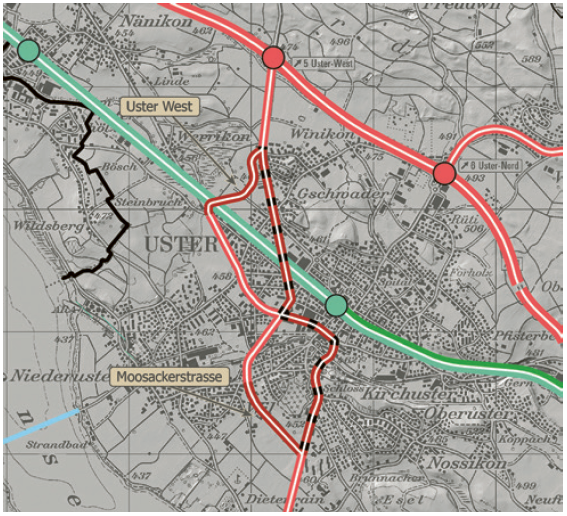
\includegraphics[width=0.6\textwidth]{figures/f-04-04-UsterWest-Moosackerstr}
	\caption[Strassenprojekte Uster]{Strassenprojekte Moosackerstrasse und Usterwest gemäss (\cite{STEK})}
	\label{img:Strassenprojekte}
\end{figure}

Die Abbildung \ref{img:Strassenprojekte} zeigt die geplanten kantonalen Strassenprojekte Usterwest und Moosackerstrasse. Durch diese Strassenprojekte, sollen einerseits die Stadterschliessung verbessert und andererseits das Zentrum vom Durchgangsverkehr entlastet werden. Insbesondere die Verkehrsbelastung des Nüsslikreis, soll durch den Bau der Moosackerstrasse reduziert werden. Gemäss dem STEK ist die Realisierung der Uster Westumfahrung in näherer Zukunft nicht absehbar. Mit dem Bau der Moosackerstrasse hingegen, kann in näherer Zukunft gerechnet werden, was zu einer Reduktion des Durchgangsverkehr im Zentrum und einer Entlastung des Nüsslikreisel führen wird. Laut dem STEK wird die Situation an den bestehenden Bahnübergängen, durch den Bau der Moosackerstrasse nicht verbessert. Um die Situation an den Bahnübergängen nachhaltig zu verbessern, muss ein anderer Lösungsansatz gefunden werden. 

\begin{figure}[h!]
	\centering
	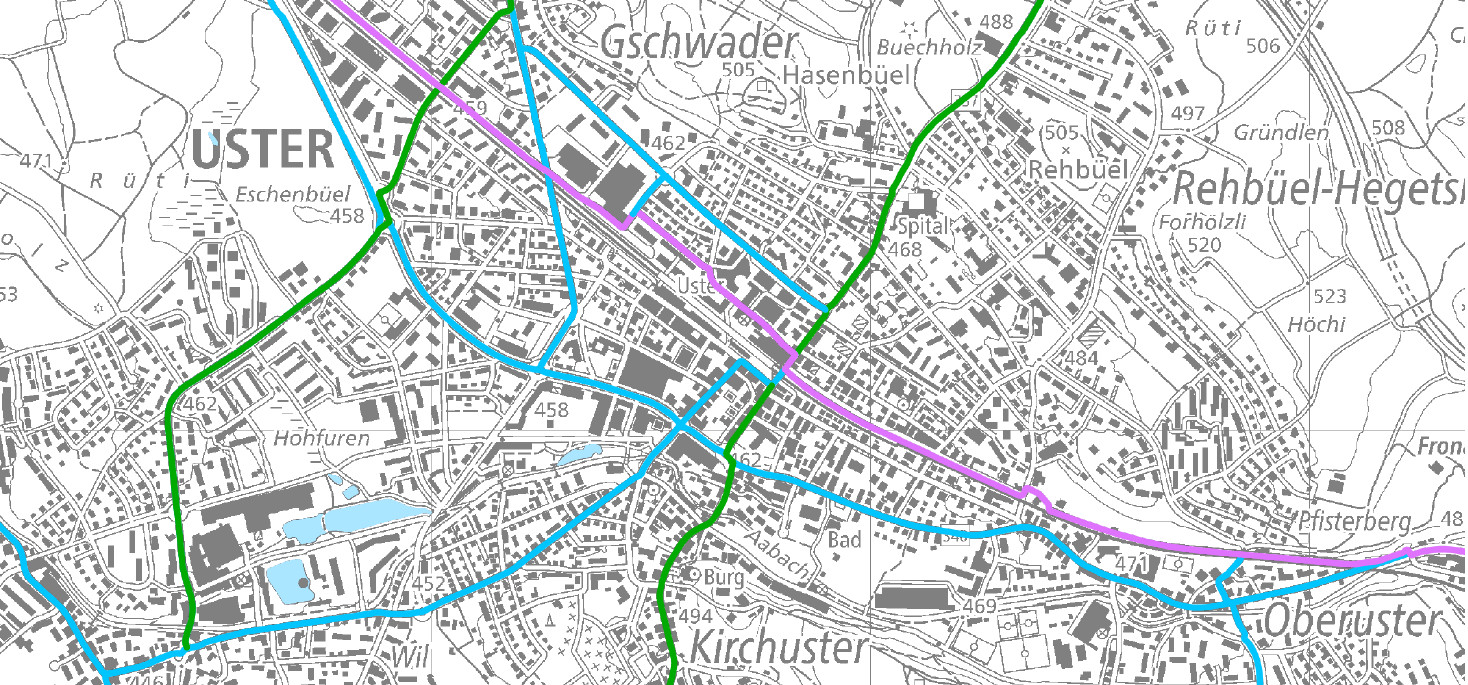
\includegraphics[width=\textwidth]{figures/f-04-01-Veloweg-Alltag}
	\caption[Velonetz Alltag]{Velonetz Alltag (\cite{GIS})}
	\label{img:Velonetz}
\end{figure}
 
Die Abbildung \ref{img:Velonetz} zeigt das Velonetz der Innenstadt von Uster. In grün sind die Hauptverbindungen, in blau die Nebenverbindungen und in violett die Veloschnellroute dargestellt. Wie in der Abbildung ersichtlich, ist der Bahnübergang Brunnenstrasse der zentrale Knotenpunkt des Velonetz. Die Gleisquerung ist für den Langsamverkehr, aufgrund des dichten S-Bahn Fahrplans, nur mit langen Wartezeiten möglich. 

Gemäss der Leitziele, die sich Uster im Rahmen der Stadtenticklung 2035 gegeben hat, soll Uster zur Velostadt ausgebaut werden. Die von der SP eingereichte Velointiative wiederspiegelt zusätzlich das Bedürfnis der Bevölkerung nach einer Förderung des Langsamverkehrs. Insbesondere die, im kantonalen Städtevergleich, als unterdurchschnittlich erachtete Dichte des Velonetz, stellt für die Bevölkerung ein Mangel dar, sowie ist die Verkehrssicherheit, aufgrund der stark am MIV ausgerichten Strassenräume, auf dem bestehenden Velonetz ungenüngend. \\

\paragraph{Fokus} 

Nach der Analyse des STEK bin ich zum Schluss gekommen, dass die Zerschneidung der Stadt durch die Gleisanlage eines der grössten Probleme von Uster darstellt. Die Verbesserung der Gleisquerung und Erhöhung der Sicherheit auf dem bestehenden Velonetz und der damit einhergehenden Erhöhung der Erreichbarkeit des Zentrums, erachte ich optimaler Ansatz, um eine Verbesserung der Verkehrssituation in Uster zu erreichen. 

Unter Anbetracht der ersten Bestrebungen der Stadt Uster den Verkehr im Zentrum zu reduzieren, sprich die Umleitung des Nord-Süd Durchgangsverkehr über die Oberlandstrasse zur Unterführung Dammstrasse, und der Leitziele des STEK "den Langsamverkehr zu fördern", habe ich mich dazu entschieden, die Situation am Bahnübergang Brunnenstrasse zu optimieren.


\begin{figure}[h!]
	\centering
	\includegraphics[width=0.6\textwidth]{figures/f-04-01-Bahnübergang-FOTO}
	\caption[Bahnübergang Brunnenstrasse]{Bahnübergang Brunnenstrasse und Velonetz Alltag (\cite{GIS})}
	\label{img:Brunnenstrasse}
\end{figure}

Die Abbildung \ref{img:Brunnenstrasse} zeigt den Bahnübergang Brunnenstrasse, die die südlich des Bahnhofs gelegenen Stadteile mit dem Spital und der Sportanlage Buchholz, sowie die nördlich des Bahnhofs gelegenen Quartiere mit dem Stadtzentrum und dem Greifensee, verbinden. 

Die im Rahmen dieser Projektarbeit generierten Optimierungsvorschläge, sollen die Verkehrssituation nachhaltig verbessern. Deshalb untersuche ich den Effekt dieser Varianten auf die Verkehrssituation über einen Zeitraum von vierzig Jahren. Um das beste Investment für die Stadt Uster, ermitteln zu können, definiere ich im nachfolgenden Abschnitt, die Ziele die mit der Intervention erreicht werden sollen.

\pagebreak

\section{Formulierung der Ziele und Rahmenbedingungen}
\label{sec:Zielformulierung}

In Anbetracht der dezentralen Struktur von Uster und der geplanten Aufwertung der Innenstadt, ist eine Verbesserung der Erreichbarkeit des Zentrums unabdingbar. Eine Verbesserung der Erreichbarkeit setzt voraus, dass die Reisezeit verkürzt und die Verkehrssicherheit erhöht wird. Durch die Umgestaltung des Bahnübergangs und der Verbesserung der Signalisation, soll der Teilung der Stadt durch die Gleisanlagen entgegengewirkt werden und so ein wichtiger Beitrag zur Stadtentwicklung geleistet werden. Dies soll eine Verkehrsberuhigung der zentrumsnahen Verkehrsnetze fördern und durch die punktuelle Aufwertung die Aufenthaltsqualität steigern.

Die von mir geplante Intervention in das bestehende Infrastrukturnetz, soll die Verkehrssituation am Bahnhof nachhaltig optimieren, sowie die Attraktivität und die Standortqualitäten von Uster stärken. Das Ziel ist, unter Berücksichtigung der unsicheren zukünftigen Gegebenheiten, der gesteigerten Nachfrage nach Mobilität Rechnung zu tragen, sowie den Langsamverkehrsanteil am Modalsplit des Innenstadtverkehrs zu beeinflussen.
 
Diese Optimierung soll, durch die minimierung der Kosten, den Gesamtnutzen aller Interessensgruppen steigern. Aufgrund dessen, dass in der nachfolgenden Berechnung, nur die Kosten der beteiligten Personen berücksichtigt werden, ist die Minimierung der Kosten mit der Maximierung des Nutzens gleichzusetzen. \\
So sollen einerseits, durch die Verkürzung der Reisezeit die Kosten der Nutzer gesenkt und durch die Erhöhung der Verkehrssicherheit die Kosten der Öffentlichkeit, reduziert werden und andererseits durch die Bestimmung der für den Zeitraum der nächsten vierzig Jahre optimalen Varianten, für die Besitzer das optimale Investment ermittelt werden.


	\subsection{Interessensgruppen}
	%=============================================================================
% Thesis Template in LaTex
%
% File:  Interessensgruppen -- Fallstudie
% Author(s): Jürgen Hackl <hackl@ibi.baug.ethz.ch>
%            Clemens Kielhauser <kielhauser@ibi.baug.ethz.ch>
%
% Creation:  27 Jan 2014
% Time-stamp: <Tue 2013-08-13 20:14 juergen>
%
% Copyright (c) 2014 Infrastructure Management Group (IMG)
%               http://ibi.ethz.ch
%
% More information on LaTeX: http://www.latex-project.org/
%=============================================================================

% Unterkapitel Interessengruppen
% ---------
\label{subsec:Gruppen}

\begin{description}
\item[Besitzer]\hfill \\
Die Interessensgruppe der Eigentümer setzt sich aus verschiedene Parteien zusammen. Die wichtigsten involvierten Parteien sind die Stadt Uster und der Kanton Zürich sowie die Eigentümerin der Sportanlage Buchholz. Sie werden durch die Baudirektion der Stadt Uster vertreten.
Für die Besitzerin der Infrastruktur wird in dem betrachteten Zeitraum nur die Initialisierungskosten sowie die laufenden Betriebskosten von Bedeutung sein. Um ein vollständiges Bild der Interessen der Besitzer zu erhalten, müssten weiter Kosten in Betracht gezogen werden. 
Für unsere Untersuchungen, welche die Infrastruktur in den nächsten 40 Jahren betrachtet, spielen die Unterhaltskosten die bedeutendste Rolle. Einerseits übersteigt die W'keit, dass diese Kosten bezahlt werden müssen, die W'keit dass andere Kostentypen eintreten und andererseits ist der absolute Betrag der Unterhaltskosten über einen Zeitraum von $T$ Jahren deutlich grössers als der anderer Kostentypen. Aufgrund dieser Überlegungen brachten wir für die Besitzer nur die Unterhaltskosten. 
\item[Nutzer]\hfill \\ 
Für die nachfolgende Optimierung ist es von zentraler Bedeutung die massgebenden Kostenstrukturen zu definieren. In anbetracht der Verkehssituation, sind die  folgenden Kostentypen diejenigen die für den Nutzer massgebenden sind. 
Der Nutzer der Infrastruktur ist der Langsamverkehr der gemäss STEK sämtliche Verkehrsmitteln einschliesst die aus eigener Kraft angetrieben werden. Es muss geprüft werden ob auch Sonderbewilligungen zur Nutzung der Infrastruktur für E-Bikes und Hybridräder erteilt werden kann. Dies sollte nur geschehen fals die geplannte Kapazität der Infrastruktur das befahren mit deutlich unterschiedlichen Geschwindigekeiten erlaubt.
Die Infrastruktur ist für jegliche Art von nichtmotorisiertem Verkehr ausgelegt. Dieser beinhaltet Fahrräder, Inlineskater, Skateboarder und auch Rollstuhlfahrer.Wichtig für die planung der Intervention ist die Unterteilung der Verkehrsteilnehmer anhand ihrer durchschnittlichen Geschwindigkeit.
\item[Öffentliche Hand]\hfill \\
Die in Tabelle \ref{tab:t-04-01-Interessensgruppen} aufgeführten Kosten sind die massgebenden Einwirkungen auf die Allgemeinheit. Die Öffentliche Hand setzt sich aus direkt und indirekt betroffener Personen zusammen. 
Die Anwohner sowie in einem entfernteren Sinne auch die Nutzer selbst, zählen zur direkt betroffenen Öffentlichkeit. Sie nutzen die Infrastruktur nicht direkt, befinden sich aber in ihrer unmittelbaren Nähe. Diese sind die Hauptträger der Kosten die durch Lärm- und Schadstoffbelastung enstehen. Eine Reduktion des MIV Anteil und die damit einhergehende verkehrsberuhigung sind die besten Mittel zur Reduktion dieser Kosten.   \\
Die Unfallkosten gehen zulasten der Allgemeinheit in Form der Belastung des Gesundheitssystems. Die Allgemeinheit nutzt in diesem Sinne die Infrastruktur nicht und ist auch nicht in ihrer Nähe zuhause oder bei der Arbeit sondern wird durch die Benützung der Infrastruktur von ihr indirekt betroffen.
\end{description}




% ===========================================================================
% EOF
%

%%% Local Variables:
%%% mode: latex
%%% TeX-master: "../main"
%%% End:


	\subsection{Zielfunktion}
	%=============================================================================
% Thesis Template in LaTex
%
% File:  Zielfunktion -- Fallstudie
% Author(s): Jürgen Hackl <hackl@ibi.baug.ethz.ch>
%            Clemens Kielhauser <kielhauser@ibi.baug.ethz.ch>
%
% Creation:  27 Jan 2014
% Time-stamp: <Tue 2013-08-13 20:14 juergen>
%
% Copyright (c) 2014 Infrastructure Management Group (IMG)
%               http://ibi.ethz.ch
%
% More information on LaTeX: http://www.latex-project.org/
%=============================================================================

% Unterkapitel Zielfunktion
% ---------
\label{subsec:Funktion}


Das Ziel meiner Optimierung ist es den Gesamtnutzen zu steigern mit speziellem Augenmerk auf der Vermehrung des Nutzens der Fahrradfahrer.

Die geplanten Infrastruktur Interventionen sollen die Kapazität und somit das Angebot auf der Route Bahnhof - Sportanlage erhöhen. 

Mithilfe der Optimierung und der anschliessenden Analyse soll diejenige Intervention bestimmt werden, die den totalen Nutzen über den betrachteten Zeitraum am meisten steigert. 


Die Gleichung \ref{equation:1} stellt das Optimierungsproblem als mathematische Funktion dar.
Die totalen Kosten $TK$ einer Interventionsstrategie sind definiert als die netto Kosten aller Steakholder über einen untersuchten Zeitraum $[0,T]$ 

Da in userem Fall die Erlöse, während einer Zeitperiode $[0,T]$ generiert werden können, nicht in Betracht gezogen werden, ist die minimierung der Gesamtkosten äquivalent zur maximierung des netto Nutzens aller beteiligter Interessensverände. 
Die Zeit $0$ kennzeichnet den Startpunkt der Untersuchung wobei die Zeit $T$ das Ende der Untersuchungsperiode ist. 

\begin{equation}
Min. \thinspace TK_{i} = Min. \thinspace [K_{U}^i + K_{TT}^i + K_{B}^i + K_{E}^i + K_{A}^i]
\label{equation:1}
\end{equation} 

{\setstretch{0.75}
wobei:
\begin{conditions}
\renewcommand{\arraystretch}{0.7}
 TK_{i}   	    &  Totale Kosten der Variante $i$ für den betrachteten Zeitraum von $T$ Jahren \\
 K_{U}^i		&  Totale Unterhalts- und Baukosten der Variante $i$ \\
 K_{TT}^i       &  Totale Reisezeitkosten der Variante $i$    \\
 K_{B}^i        &  Totale Betriebskosten der Variante $i$ \\
 K_{E}^i	    &  Totale Umweltbelastungskosten der Variante $i$  \\
 K_{A}^i        &  Totale Unfallkosten der Variante $i$ 
\end{conditions}
}

Tabelle \ref{tab:t-04-01-Interessensgruppen} listet die Interessensgruppen sowie die Kostenstrukturen auf. Die Kostenstrukturen in Form der Kostentypen und der modelierten Einheitskosten werden in den folgenden Kapitel erläutert .

%=============================================================================
% Thesis Template in LaTex
%
% File:  t-05-01-IsingModel.tex -- Table for the Ising
% Author(s): Juergen Hackl <hackl@ibi.baug.ethz.ch>
%            Clemens Kielhauser <kielhauser@ibi.baug.ethz.ch>
%
% Creation:  27 Jan 2014
% Time-stamp: <Tue 2013-08-13 20:14 juergen>
%
% Copyright (c) 2014 Infrastructure Management Group (IMG)
%               http://ibi.ethz.ch
%
% More information on LaTeX: http://www.latex-project.org/
%=============================================================================

\begin{table}[ht!]
\flushleft
\renewcommand{\arraystretch}{1.4}
%\small\renewcommand{\arraystretch}{1.2} 
%
%
\begin{tabular}{@{}p{3.3cm} p{4cm} p{1.2cm} r l @{}} \\   
\toprule
\textbf{Interessensgruppe} & \textbf{Kostentyp} & \textbf{Symbol} & \multicolumn{2}{c}{\textbf{Einheitskosten}} 			\\
\midrule
Besitzer                   & Unterhaltkosten (\textit{U})                    & $K_{U}(t)$    & 5 - 30 		&	$\frac{CHF}{m^2 \ Jahr}$              \\
Nutzer		               & Reisezeitkosten (\textit{TT})                   & $K_{TT}(t)$   & 35 - 56 		&	$\frac{CHF}{Stunde \ DTV_{k}}$         \\
                           & Betriebskosten (\textit{B})            		 & $K_{B}(t)$    & 0.15 - 0.7 	&	$\frac{CHF}{km \ DTV_{k}}$              \\
Öffentliche Hand           & Kosten durch Belastung \newline der Umwelt \newline (Environment) (\textit{E})   & $K_{E}(t)$    & 0.05  & $\frac{CHF}{Fahrzeugkilometer}$      \\
                           & Unfallkosten (\textit{A})                       & $K_{A}(t)$    & 15'000 - 3.7mio & $\frac{CHF}{Unfall_{n}}$    \\
\bottomrule

\end{tabular}
\caption{Tabelle der Interessensgruppen und Kostenstrukturen}
\label{tab:t-04-01-Interessensgruppen}
\end{table}


%=============================================================================
% EOF
%

%%% Local Variables:
%%% mode: latex
%%% TeX-master: "../guidelines"
%%% End:



\newpage

% ===========================================================================
% EOF
%

%%% Local Variables:
%%% mode: latex
%%% TeX-master: "../main"
%%% End:

	
\pagebreak

\section{Kostenstruktur}
\label{sec:Kostenstruktur}

Um das Risiko das von der Durchgführung einer Intervention ausgeht, berechnen zu können, muss die verwendete Kostenstruktur definiert werden. 
Im allgemeinen erfolgt die approximation der Kosten durch die Bestimmung der relevanten Faktoren, wie zum Beispiel der Länge und der Breite der Infrastruktur, des täglichen Verkehrsaufkommens, der benötigten Reisezeiten sowie weiterer Faktoren. Die ermittlung der Kosten erfolgt im Anschluss durch die Multiplikation dieser Faktoren mit den dazugehörigen Einheitskosten. (\cite{Adey2012}) 

%=============================================================================
% Thesis Template in LaTex
%
% File:  Kostenstruktur -- Fallstudie
% Author(s): Jürgen Hackl <hackl@ibi.baug.ethz.ch>
%            Clemens Kielhauser <kielhauser@ibi.baug.ethz.ch>
%
% Creation:  27 Jan 2014
% Time-stamp: <Tue 2013-08-13 20:14 juergen>
%
% Copyright (c) 2014 Infrastructure Management Group (IMG)
%               http://ibi.ethz.ch
%
% More information on LaTeX: http://www.latex-project.org/
%=============================================================================

% Unterkapitel Kostenstruktur
% ---------
\label{subsec:Kosten}

\newpage

In diesem Kapitel werden die Kosten, die für die verschienden Interessensverbände enstehen, erläutert und ihre Berechnung dargestellt.  \\
Um das Risiko, welches von einer Infrastruktur Intervention ausgeht, berechnen zu können, muss die verwendete Kostenstruktur definiert werden. 
Im allgemeinen erfolgt die approximation der Kosten durch die Bestimmung der relevanten Faktoren wie zum Beispiel der Länge und der Breite der Infrastruktur, des täglichen Verkehrsaufkommens, der benötigten Reisezeit sowie weiterer Faktoren. Die ermittlung der Kosten erfolgt im Anschluss durch die Multiplikation dieser Faktoren mit den dazugehörigen Einheitskosten.\footcite{Adey2012} \\
Die von 


\subsubsection{Unterhaltskosten}
\label{subsub:Unterhalt}

Die Berechnung der Unterhaltskosten $K_{U}$ der Infrastruktur werden in Formel \ref{eq.2} dargestellt. Sie setzen sich zusammen aus den einmaligen Investitionskosten für den Bau der Infrastruktur $K_{Bau}$ und den jährlich anfallenden Wartungskosten $K_{Wartung,t}$ gemäss Formel \ref{eq.3}. Die Baukosten und die Einheitskosten der Wartung werden nachfolgend erläutert.


\begin{align}
K_{U} &= K_{Bau} + \sum_{t=0}^T \  K_{Wartung,t}  \label{eq.2} \\
K_{Wartung,t} &= \sum_{t=1}^2 \ EK_{Wartung,k} \cdot s_{k} \cdot b_{k}  \label{eq.3} 
\end{align}

\begin{align*}
	  k &=
      \begin{cases}
        \begin{aligned}
          & 1 \\
          & 2
        \end{aligned} &
        \begin{aligned}
         & \text{für}\ \thinspace \\
         & \text{für}\ \thinspace
        \end{aligned}
        \begin{aligned}
          & Strasse \\
          & Unterfu"hrung
        \end{aligned}
      \end{cases} \\
\end{align*}

{\setstretch{0.6}
wobei:
\begin{conditions}
 K_{U}      	     			&  Totale Unterhaltskosten für $T$ Jahre  \\
 K_{Bau}           			    &  Baukosten der Variante     \\
 K_{Wartung,t}                  &  Wartungskosten pro Jahr     \\
 EK_{Wartung,k}      	     	&  Einheitskosten pro $m^2$   \\
 s_k	    	     			&  Länge der Infrastruktur in $m$ \\
 b_k	    	     			&  Breite der Infrastruktur in $m$   \\
 k								&  Art der Infrastruktur  
\end{conditions}
}

Die entstehenden Investitionskosten für den Bau der verschiedenen Instrastrukturen, habe ich nach \cite{Baukosten2010} folgendermassen angesetzt. Die Erstellung zweier neuer Radstreifen à $1.5 \, m$ Breite kostet $850 \, CHF$ pro Laufmeter. Die Investitionskosten pro Quadratmeter für den Bau einer Velounterführung unter dem Lastfall Eisenbahn, betragen $3750 \, CHF$. Der Bau der Zufahrtsrampen zu den Velounterführungen kostet pro Rampe $130'000 \, CHF$. 
Die Wartungskosten der verschiedenen Infrastruktur Typen habe ich nach einem Gespräch mit Herr Dr. Martani wie folgt angesetzt. Für die Instandhaltung der Strasse, inklusive der Fahrradstreifen und der Fussgängerwege nehme ich an, dass jährlich $5 \thinspace \frac{CHF}{m^2}$ anfallen. Die wartungsintesivere Infrastruktur der Unterführung wird jährlich mit $30 \thinspace \frac{CHF}{m^2}$ instand gehalten.  

\newpage

\subsubsection{Reisezeitkosten}
\label{subsub:Reisezeit}


Die beim benutzen der Infrastruktur enstehenden Reisezeitkosten ($TT$) (engl. Travel time cost), spiegeln die wirtschaftlichen Auswirkungen des Zeitverlustes auf den Verkehrsteilnehmer wieder und sind somit die Kosten der Reise in Form von Zeitverlust. In Anbetracht der Tatsache, dass in dieser verlorenen Zeit gearbeitet, sowie Freizeit verbracht hätte werden können, kann dieser Zeitverlust monetär beziffert werden. Dies erfolgt mit den nachfolgen beschriebenen Einheitskosten des Zeitverlustes.  
Die Berechnung der totalen Reisezeitkosten $K_{TT}$ für $T$ Jahre erfolgt gemäss Formel \ref{eq.4} und ist eine Vereinfachung der Berechnung der \textit{Travel time cost} \cite[vlg.][643]{Adey2012}.
  

\begin{align}
K_{TT} &= \sum_{t=0}^T \Biggl[ \sum_{j=1}^2 \ DTV_{j} \cdot t_{j} \cdot EK_{TT,j} \Biggr] \label{eq.4} \\
t &= \frac{s_{k}}{v_{j}} \Biggl( 1 + 0.15 \Bigl(\frac{DTV_{j}}{C_{j}} \Bigr)^4 \Biggr) \label{eg.5} 
\end{align}

\begin{align*}
	 j &=
      \begin{cases}
        \begin{aligned}
          & 1 \\
          & 2
        \end{aligned} &
        \begin{aligned}
         & \text{für}\ \thinspace \\
         & \text{für}\ \thinspace
        \end{aligned}
        \begin{aligned}
          & für MIV \\
          & für Velo
        \end{aligned}
      \end{cases} \\
\end{align*}

{\setstretch{0.75}
wobei:
\begin{conditions}
 K_{TT}		 	 &  Totale Reisezeitkosten für $T$ Jahre  \\
 DTV_{j}    	 &  Tägliches Verkehrsaufkommen nach Fahrzeugtyp \\
 t_{j} 			 &  Zeitverlust nach Fahrzeugtyp \\
 EK_{TT,j} 		 &  Einheitskosten der verlorenen Zeit  \\
 v_{j}			 &  Gefahrene Geschwindigkeit nach Fahrzeugtyp \\
 C_{j}			 &  Kapazität der Infrastruktur nach Fahrzeugtyp  \\
 j				 &  Art des Fahrzeugs   
\end{conditions}
}

Der Zeitverlust ist abhängig vom Zustand der Infrastruktur, genauer von der Beschaffenheit des Oberflächenbelags der Fahrbahn. sowie der momentanen Auslastung. Diese Beziehungen ist schwierig zu modelieren. Jedoch kann zwischen dem Zeitverlust auf der Infrastruktur, dem Auslastungsgrad, in Abhängigkeit von der gebauten Variante und der gefahrenen Geschwindigkeit eine Beziehung modeliert werden. Diese Approximation ermöglicht es mir, die verlorene Zeit, gemäss \ref{eg.5} zu berechnen.  
Die Zeit die man benötigt eine bestimmte Strecke zurück zu legen ist abhängig von der gefahrenen Geschwindigkeit welche wiederum abhängig ist vom Zustand der Strasse sowie der Kapazität der Infrastruktur. Wird die Kapazität durch eine zu hohe Nachfrage überschritten, kann dies zu einer Überlastung des Systems führen und somit zu Verstopfungen und daraus resultierenden Verspätungen.  

Die Einheitskosten der verlorenen Zeit $EK_{TT,j}$ werden anhand des schweizerischen Medianlohn von 2018 berechnet. Der Medianlohn betrug im Jahr 2018 $6538 \, CHF$ pro Monat bei einer durchschnittlichen Arbeitszeit von 42,5 Stunden pro Woche (Quelle: BFS). Daraus ergibt sich einen durchschnittlichen Bruttostundenlohn von $38,5 \, CHF/h$ pro Person, was im Falle dieser Berechnung den Einheitskosten der verlorenen Reisezeit eines Velofahrers entspricht. Unter der Annahme eines durchschnittlichen Auslastungsgrad von 1.6 Personen pro Fahrzeuge \cite{Mikrozensus2015}, betragen die Einheitskosten der verlorenen Reisezeit pro Fahrzeug $61,6 \, CHF/h$.



\subsubsection{Betriebskosten}
\label{subsub:Betrieb}


Die Betriebskosten $K_{B}$ die für die Nutzer der Infrastruktur, für den betrachteten Zeitraum von $T$ Jahren, anfallen, werden gemäss Formel \ref{eq.6} berechnet. So werden die Betriebskosten aus der Multiplikation der Anzahl Nutzer und der zurückgelegten Distanz mit den Einheitskosten pro Fahrzeugkilometer ermittelt.
Diese sogenannten Fahrzeugsbetriebkosten sind im Rahmen dieser Optimierung, als die jährlich pro Nutzer anfallenden Wartungskosten definiert und sind somit die Kosten, die für die Instandsetzung und den Betrieb eines Fahrzeugs, bei benützung der Infrastruktur, entstehen können. Diese setzen sich zusammen aus den Kosten der Arbeitssstunden für die Instandsetzung sowie der Kosten für die Ersatz- und Verschleissteile.
 
Diese Kosten sind abhängig von der Qualität des Fahrbahnbelags, von der Ausführung der Infrastruktur und von der Kapazität der Infrastruktur. Weiter ist ein entscheidender Faktor in der Bestimmung der Fahrzeugbetriebskosten die Strassengeometry. Diese beinhaltet die Anzahl und Form der Kurven, die Steigungen sowie die Breite der Strasse und die daraus resultierende Möglichkeit des sicheren Überholens. Die Anzahl an Kreuzungsstellen und die davon abhänginge Anzahl an Brems- und Beschleunigungsmanöver haben einen direkten Einfluss auf den Verschleiss der Mechanik des Fahrzeugs. So werden im Falle des Fahrrads die Kette und die Bremsbeläge durch vermehrtes Bremsen und Anfahren verstärkt abgenutzt und im Falle des Autos erhöhen sich die Betriebskosten bei vermehrtem \textit{Stop-and-Go} Verkehr.

\begin{equation}
K_{B} =  \sum_{t=0}^T \Biggl[ \sum_{j=1}^2 \ EK_{B,j} \cdot s_{k} \cdot DTV_{j} \Biggr]  \label{eq.6} \\
\end{equation}

{\setstretch{0.75}
wobei:
\begin{conditions}
 K_{B}			   &  Totale Fahrzeugbetriebskosten \\
 EK_{B,j}	       &  Einheitskosten pro $km$ \\
 s_j	    	   &  Länge der Infrastruktur nach Fahrzeugtyp in $km$ 
\end{conditions}
}

Zur Vereinfachung der Berechnung, werden die entstehenden Betriebskosten anhand der nachfolgenden Referenzwerte ermittelt.
Die Kosten der Arbeitsstunden sowie die Kosten der Materialien werden zusammengefasst als die Einheitskosten $EK_{B}$ für den Fahrzeugbetrieb.
Diese betragen pro Auto $0.7 CHF$ pro $km$ und pro Velo $0.15 CHF$ pro $km$ (Quelle: TCS). 

\newpage


\subsubsection{Kosten durch Belastung der Umwelt}
\label{subsubsec:Environment}


Die Kosten die durch die Belastung der Umwelt $K_{E}(t)$ (\textit{Englisch}: Environment) entstehen,
setzen sich auf den Kosten der Luftverschmutzung durch die Schadstoffbelastung $K_{S}$ und der Kosten durch die Lärmbelastung $K_{L}$ zusammen und werden gemäss Formel \ref{eq.7} berechnet. 

Die Kosten durch die Schadstoffbelastung $K_{S}$, sind die Kosten die für die Allgemeinheit durch die Schäden aufgrund der Emissionen der motorisierten Fahrzeuge, entstehen können. Diese Schäden können neben gesundheitlichen Problemen für die Anwohner und Nutzer der Strasse auch die Beeinträchtigung des Pflanzenwachstums entlang der Infrastruktur, sowie die Reduktion des Wertes der Liegenschaft sein. 
Die Kosten durch die Lärmbelastung $K_{L}$, sind die Kosten die für die Allgemeinheit durch übermässigen Lärm, welcher von der Strasse verursacht wird, entstehen können. 
Die Kosten sind in diesem Falle die Störung und Beeinträchtigung der Anwohner in Form von Kopfschmerzen, Bluthochdruck, Schlafstörrungen sowie psychischer Belastung. \\
Der Lärm entsteht mehrheitlich durch Motorengeräusche sowie der Abrollgeräusche der Reifen. \cite{Adey2012}

\begin{equation}
K_{E}(t) = \sum_{t=0}^T \ \biggl(K_{S,t} + K_{L,t} \biggr)  \label{eq.7} \\
\end{equation}

{\setstretch{0.75}
wobei:
\begin{conditions}
 K_{E}		   &  Totale Umwelkosten  \\
 K_{S,t}       &  Kosten durch die Schadstoffbelastung pro Jahr \\
 K_{L,t}       &  Kosten durch die Lärmbelastung pro Jahr  
\end{conditions} 
}

Die Kosten durch die \textbf{Schadstoffbelastung} werden gemäss Formel \ref{eq.8} berechnet.

\begin{equation}
K_{S,t} = EK_{S} \cdot DTV_{MIV,t} \cdot s_{i} \biggl( 1 - \Phi_{E-Auto,t} \biggr)   \label{eq.8} \\
\end{equation}

{\setstretch{0.75}
wobei:
\begin{conditions}
 EK_{S}         	&  Einheitskosten der Schadstoffbelastug pro Fahrzeugkilometer \\
 DTV_{MIV,t}    	&  Durchschnittliche tägliche Verkehrsaufkommen des MIV im Jahr $t$  \\
 s_{MIV}          	&  Zurückgelegte Distanz in $[km]$ \\
 \Phi_{E-Auto,t}    &  Marktanteil E-Autos am $DTV_{MIV,t}$ im Jahr $t$ 
\end{conditions} 
}

Die Kosten durch die \textbf{Lärmbelastung} werden gemäss Formel \ref{eq.9} berechnet.

\begin{equation}
K_{L,t} = EK_{L} \cdot DTV_{MIV,t} \cdot s_{i}  \label{eq.9} \\
\end{equation}

{\setstretch{0.75}
wobei:
\begin{conditions}
 EK_{L}         	&  Einheitskosten der Lärmbelastung pro Fahrzeugkilometer \\
 DTV_{MIV,t}    	&  Durchschnittliche tägliche Verkehrsaufkommen im Jahr $t$  \\
 s_{MIV}          	&  Zurückgelegte Distanz in $[km]$ pro Fahrzeug 
\end{conditions} 
}

Die Schadstoffbelastung ist eine Funktion der durchschnittlich gefahrenen Geschwindigkeit sowie der Häufigkeit des \textit{Stopp and Go - Verkehrs}. So nimmt die Belastung der Luft durch Schadstoffe deutlich zu, wenn vermehrt im \textit{Stopp and Go - Verkehr} gefahren wird. 
Da diese Beziehung schwierig zu modelieren ist, wird im Rahmen dieser Untersuchung die Einheitskosten der Schadstoffbelastung $EK_{S}$ pro Fahrzeugkilometer gemäss \cite[p.38]{Ecoplan2007} mit $0.0345 \, CHF/Fahrzeugkilometer$ angesetzt. \\
Die Einheitskosten der Lärmbelastung $EK_{L}$ werden gemäss \cite[p.127]{Lärm2000} mit $0.0149 \, CHF/Fahrzeugkilometer$ angenähert. 


\subsubsection{Unfallkosten}
\label{subsubsec:Unfall}


Die totalen Unfallkosten $K_{A}$ welche von der Allgemeinheit für den betrachteten Zeitraum von $T$ Jahren getragen werden müssen, werden gemäss Formel \ref{eq.10} berechnet. \\
Die Berechnung dieser Kosten basiert auf der Kostenberechnung in \cite{Adey2012}.
In Betracht gezogen werden drei verschiedene Unfaltypen [$a$,$b$,$c$].
Unfälle mit entstandenen Sachschäden und leichtverletzten Personen werden in die Kategorie $a$ eingeteilt. Für Unfälle mit schwerverletzten Beteiligten wird die Kategorie $b$ definiert und für Unfälle mit Todesfolge die Kategorie $c$. 
Die Kategorien unterscheidenen sich in der Häufigkeit des Unfalls pro Fahrzeug \( \gamma_{j,n} \) sowie der entstehenden Einheitskosten pro Unfall $EK_{j,n}$. \\
Die pro Unfall entstehenden Einheitskosten sowie die Unfallhäufigkeiten werden nachfolgend erläutert.
Wichtig anzumerken ist, dass die ermittelten Unfallrisiken die Anzahl Unfälle eines Unfalltyps pro Personenkilometer darstellen. Das bedeuted, dass für die Berechnung der Personenkilometer der mototrisierten Fahrzeuge, der Auslastungsgrad gemäss \cite{Mikrozensus2015} in Betracht gezogen werden muss. Somit wird in der Berechnung der Unfallkosten der $DTV_{MIV}$ mit einem Faktor 1.6 multipliziert.

\begin{equation}
K_{A} = \sum_{t=0}^T \Biggl[ \sum_{j=1}^2 \Bigl( \sum_{n=a}^c \ EK_{j,n} \cdot \gamma_{j,n} \Bigr) \cdot DTV_{j} \cdot s_j \Biggr] 
\label{eq.10}
\end{equation}

\begin{align*}
      n &=
      \begin{cases}
        \begin{aligned}
          & a  \\
          & b \\
          & c
        \end{aligned} &
        \begin{aligned}
         & \text{für}\ \thinspace \\
         & \text{für}\ \thinspace \\
         & \text{für}\ \thinspace
        \end{aligned}
        \begin{aligned}
          & {Sachsch"aden\,und\,Leichtverletzte} \\
          & {Schwerverletzte} \\
          & {Todesfall}
        \end{aligned}
      \end{cases}  \\
      j &=
      \begin{cases}
        \begin{aligned}
          & 1 \\
          & 2
        \end{aligned} &
        \begin{aligned}
         & \text{für}\ \thinspace \\
         & \text{für}\ \thinspace
        \end{aligned}
        \begin{aligned}
          & Velo \\
          & Auto
        \end{aligned}
      \end{cases} \\
\end{align*}

{\setstretch{0.75}
wobei:
\begin{conditions}
 K_{A}	 		 &  Totale Unfallkosten \\
 EK_{j,n} 		 &  Einheitskosten pro Unfall nach Fahrzeugtyp \\
 \gamma_{j,n} 	 &  Unfallwahrscheinlichkeit nach Fahrzeugtyp \\
 DTV_{j}		 &  Tägliches Verkehrsaufkommen nach Fahrzeugtyp \\
 s_j	    	 &  Länge der Infrastruktur nach Fahrzeugtyp in $km$  \\
 n 				 &  Unfallart  \\
 j          	 &  Art des Fahrzeugs  
\end{conditions}
} 

Die Anzahl Unfälle pro Personenkilometer und somit die Unfallwahrscheinlichkeit \( \gamma_{j,n} \) wird mithilfe der Risiken eines Unfall mit Todesfolge gemäss \cite{Unfallrisiko2019} ermittelt. 
So betrug das Sterberisiko pro zurückgelegter Distanz von 2008 bis 2017 für einen Personenwagen; ein Todesfall pro 828 Mio. Personenkilometer (Quelle: BFS). Aus diesem Risiko ermittle ich die Unfallwahrscheinlichkeit eines Unfalls mit Todesfolge, was beudeuted, dass ich die Anzahl Unfälle mit Todesfolge pro einem Personenkilometer ermittle. 
Um die Berechnung zu vereinfachen habe ich die Personenwagen und die Motorräder unter der Bezeichnung MIV zusammengefasst. Um der höheren Unfallwahrscheinlichkeit der Motorradfahrer rechnung zu tragen, habe ich die Unfallwahrscheinlichkeit des MIV wie folgt ermittelt. \\
$\gamma_{MIV,c} = Anteil_{Motorrad} \cdot \gamma_{Motorrad,c} + Anteil_{Auto,c} \cdot \gamma_{Auto,c}$ \\
Somit wurde der prozentuale Anteil an der Gesamtmenge an Strassenmotorfahrzeugen verwendet um das Unfallrisiko des MIV's zu berechnen.
Die Anzahl Strassenmotorfahrzeuge in der Schweiz betrug 2019 6'160'262 Fahrzeuge.\footcite[Vlg.]{Bestand2019}
Davon waren 744'542 Motorräder, was einem Anteil von 12.09\% entspricht. Der Rest wird in dieser Betrachtung als Autos definiert. 

Die Berechnung der Unfallrisiken der Unfalltypen $a$ und $b$ erfolgte mithilfe des prozentualen Anteile dieser Unfalltypen an der Gesamtanzahl an Unfällen im Jahr 2019. Die Unfallrisiken der Unfalltypen $a$ und $b$ wurden somit mithilfer dieser Anteile aus dem Unfallrisiko für die Unfälle des Typs $c$ geschätzt.
Die Anzahl Unfälle der verschiedenen Typen wird der Strassenverkehrsunfall-Statistik des Bundesamt für Strassen entnommen und die Werte beziehen sich auf das Jahr 2019.
So waren 2019 0.334\% aller Unfälle, Unfälle mit Todesfolge, 6.45\% aller Unfäller waren Unfälle mit Schwerverletzten und 93.21\% der Unfälle haten Sachschaden und Leichtverletzte Personen zur Folge.\footcite{Unfall2019}
Die ausführliche Berechnung der Unfallrisiken ist im Anhang unter \ref{subsec:Unfallrisiko} dargestellt.
Die nachfolgenden Tabelle \ref{tab:t-06-01-Unfallrisiko} listet die berechneten Unfallrisiken für die verschiedenen Fahrzeuge $j$ und die verschiedenen Unfalltypen $n$ auf. 

%=============================================================================
% Thesis Template in LaTex
%
% File:  t-05-01-IsingModel.tex -- Table for the Ising
% Author(s): Juergen Hackl <hackl@ibi.baug.ethz.ch>
%            Clemens Kielhauser <kielhauser@ibi.baug.ethz.ch>
%
% Creation:  27 Jan 2014
% Time-stamp: <Tue 2013-08-13 20:14 juergen>
%
% Copyright (c) 2014 Infrastructure Management Group (IMG)
%               http://ibi.ethz.ch
%
% More information on LaTeX: http://www.latex-project.org/
%=============================================================================

\begin{table}[hbt!]
\center
%\small\renewcommand{\arraystretch}{1.2} 
%
%
\begin{tabular}{@{}p{2.6cm} p{3.3cm} p{3.3cm} p{3.3cm}@{}} \\   
\toprule
\textbf{Fahrezugtyp\textsubscript{k}} & \textbf{Unfalltyp\,a} & \textbf{Unfalltyp\,b} & \textbf{Unfalltyp\,c} \\
\midrule
MIV      & \(1.317\,\mathrm{10^{-6}}\) $\frac{Unf"alle}{Pkm}$ & \(9.116\,\mathrm{10^{-8}}\) $\frac{Unf"alle}{Pkm}$ & \(4.7243\,\mathrm{10^{-9}}\) $\frac{Unf"alle}{Pkm}$ \\
Velo	 & \(3.818\,\mathrm{10^{-6}}\)  $\frac{Unf"alle}{Pkm}$ & \(2.643\,\mathrm{10^{-7}}\)  $\frac{Unf"alle}{Pkm}$ & \(1.37\,\mathrm{10^{-8}}\)  $\frac{Unf"alle}{Pkm}$  \\

\bottomrule

\end{tabular}
\caption[Tabelle der Unfallrisiken]{Tabelle der Unfallrisiken $\gamma_{k,n}\,\Bigl[\frac{Unf"alle_{k,n}}{Pkm_{k}}\Bigl]$}
\label{tab:t-06-01-Unfallrisiko}
\end{table}


%=============================================================================
% EOF
%

%%% Local Variables:
%%% mode: latex
%%% TeX-master: "../guidelines"
%%% End:



\newpage

Nach der ausführlichen Betrachtung verschiedenster Literatur zum Thema: \textit{Kosten die durch Strassenverkehrsunfälle entstehen} und einem Gespräch mit Herr Dr. Martani habe ich für die Berechnung der Unfallkosten im Rahmen dieser Untersuchung die folgenden Einheitskosten der verschiedenen Unfalltypen festgelegt.


\paragraph{Katergorie $a$} Die Einheitskosten pro Unfall der Kategorie $a$ setzen sich aus den entstandenen Sachschäden und den Arbeits- und Materialkösten der Reperatur der Fahrzeuge zusammen. Unter der Annahme, dass das durchschnittliche Alter eines Personenenwagens in der Schweiz 8.5 Jahre beträgt und somit schon einen deutlichen Wertverlust erlitten hat, werden die enstehenden Einheitskosten der Kategorie $a$ mit $15'000 CHF/Unfall$ angesetzt. Die Kosten für die Behandlung leichtverletzter Personen wird in dieser Betrachtung aufgrund ihrer geringen grösse vernachlässigt.

\paragraph{Kategorie $b$} Die Einheitskosten die aufgrund der Unfälle der Kategorie $b$ entstehen, werden durch die anfallenden Behandlungskosten der verunfallten Person dominiert. Die entstehenden Kosten durch den Erwerbsausfall für die Dauer der Arbeitsunfähigkeit sowie die Kosten der entstandenen Sachschäden werden in dieser Berechnung aufgrund ihrer im Vergleich zu den Behandlungskosten geringen Grösse, vernachlässigt. Die durchschnittliche Kosten die durch eine schwerverletzte Person entstehen, werden mit $110'000 CHF/Unfall$ angesetzt. Dies entspricht 3\% der Kosten einer tödlich verunfallten Person.

\paragraph{Kategorie $c$} Und zuletzt die Einheitskosten für die Folgen eines Unfalls der Kategorie $c$. Diese Kosten, für einen Unfall mit Todesfolge, basieren auf der Schätzung des Werts eines statistischen Lebens. Hierfür werden $3.7mio CHF/Unfall$ angesetzt (Quelle: ASTRA).






% ===========================================================================
% EOF
%

%%% Local Variables:
%%% mode: latex
%%% TeX-master: "../main"
%%% End:

	
	
	\subsection{Unsichere Einflussfaktoren}
	\label{subsec:Uncertain}
	%=============================================================================
% Thesis Template in LaTex
%
% File:  Unsichere Parameter -- Fallstudie
% Author(s): Jürgen Hackl <hackl@ibi.baug.ethz.ch>
%            Clemens Kielhauser <kielhauser@ibi.baug.ethz.ch>
%
% Creation:  27 Jan 2014
% Time-stamp: <Tue 2013-08-13 20:14 juergen>
%
% Copyright (c) 2014 Infrastructure Management Group (IMG)
%               http://ibi.ethz.ch
%
% More information on LaTeX: http://www.latex-project.org/
%=============================================================================

% Unterkapitel Unsichere Parameter
% ---------

%\subsubsection*{Tägliches Verkehrsaufkommen}
%\label{subsubsec:DTV}

Um einen nachhaltige Verbesserung der Verkehrsproblematik in Uster zu erreichen, muss die optimale Lösung die Situation für die nächsten vierzig Jahre verbessern. Damit ein Zeitraum von vierzig Jahren untersucht werden kann, müssen die unsicheren zukünftigen Entwicklungen der wichtigsten Einflussfaktoren berücksichtigt werden. Die nachfolgende Auflistung stellt die wichtigsten Einflüsse auf die Verkehrssituation am Bahnübergang und somit auf das DTV dar. 

{\setstretch{0.6}
\begin{itemize}
\item Bevölkerungswachstum
\item Zentrumsentwicklung und Verkehrsberuhigung
\item Ausbau der Veloparkieranlagen am Bahnhof 
\item Aufwertung der Quartiere nördlich des Bahnhofs
\item Urbane Strassenraumgestaltung im Zentrumsgebiet
\item Förderung des Langsamverkehrs gemäss STEK 
\item Ausbau des Spital und der Sportanlage Buchholz
\end{itemize}
}

Alle diese Einflussfaktoren haben gemeinsam, dass einerseits ihre zukünftige Entwicklung und andererseits das Ausmass, in dem sie den DTV in der Zukunft beeinflussen, ungewiss sind. Diese Einflüsse müssen, um die Unsicherheiten hinsichtlich der zukünftigen Mobilitätssituation am Bahnübergang zu berücksichtigen und um eine optimale Lösung für die nächsten vierzig Jahre zu finden, im Rahmen dieser Optimierung modelliert werden. 

Da der Verkehr am Bahnübergang hauptsächlich aus Ziel- und Quellverkehr des Zentrums besteht, hat das Bevölkerungswachstum den grössten Einfluss auf das DTV am Bahnübergang. Gemäss STEK, leben in Uster 35'000 Einwohner. Die zu erwartende Entwicklung der Bevölkerung ist abhängig von verschiedenen Faktoren und demnach nur anhand von Prognosen vorhersagbar. Gemäss der Prognosen im STEK wird der Wachstumstrend in Zukunft anhalten. (\cite{STEK})

Der Bau der Uster Westumfahrung sowie der Bau der Moosackerstrasse haben gemäss STEK keinen nennenswerten Einfluss auf die Menge an Autos, die den Bahnübergang Brunnenstrasse in Zukunft passieren werden. Dies folgt, wie im ersten Abschnitt des Kapitel \ref{chap:Fallstudie} erläutert, der Annahme, dass die Umleitung des Durchgangsverkehr über die Oberlandstrasse bereits nahezu vollständig vollzogen ist und dass der gemessene DTV hauptsächlich aus Quell- und Zielverkehr ins Zentrums besteht.  (\cite{STEK})

\newpage


% ===========================================================================
% EOF
%

%%% Local Variables:
%%% mode: latex
%%% TeX-master: "../main"
%%% End:



%-----------------------

\section{Generierung möglicher Lösungen}
\label{sec:Varianten}
%=============================================================================
% Thesis Template in LaTex
%
% File:  Varianten -- Fallstudie
% Author(s): Jürgen Hackl <hackl@ibi.baug.ethz.ch>
%            Clemens Kielhauser <kielhauser@ibi.baug.ethz.ch>
%
% Creation:  27 Jan 2014
% Time-stamp: <Tue 2013-08-13 20:14 juergen>
%
% Copyright (c) 2014 Infrastructure Management Group (IMG)
%               http://ibi.ethz.ch
%
% More information on LaTeX: http://www.latex-project.org/
%=============================================================================

% Unterkapitel Varianten
% ---------

Die folgenden Varianten habe ich im Rahmen der Optimierung der Verkehrssituation am Bahnübergang Brunnenstrasse erarbeitet, um die Situation für die nächsten vierzig Jahre nachhaltig zu verbessern. Anschliessend an die Darstellung der Varianten folgt eine Übersicht der wichtigsten Eigenschaften und Parameter der Infrastrukturen, die für die Berechnung der Kosten verwendet werden. \\
Die Gesamtlänge des betrachteten Infrastrukturabschnitts beträgt für alle Varianten 80 Meter.


\subsection{Variante: \ 1}
\label{subsec:V1}
	
Die Variante 1 stellt den Ist-Zustand der Infrastruktur dar. In dieser Variante beträgt die durchschnittliche Wartezeit pro Nutzer, wie in Abschnitt \ref{sub:Reisezeit} erläutert, 5 Minuten.  Mit dieser Variante kann der jetzige Zustand der Infrastruktur über den betrachteten Zeitraum von vierzig Jahren untersucht werden und so die Option \flqq keine Veränderung durchführen\frqq \, überprüft werden. 

%\begin{figure}[h!]
  %\centering
  %\subfloat[][]{\label{img:V1Ü}\includegraphics[width=.6\textwidth]{./figures/1}}
  %\hfill
 % \subfloat[][]{\label{img:V1Q}\includegraphics[width=.4\textwidth]{./figures/1_2}}
%\caption[Variante 1]{Übersicht und Querschnitt der Variante 1}
 % \label{fig:V1}
%\end{figure}

\begin{figure}[h!]
	\centering
	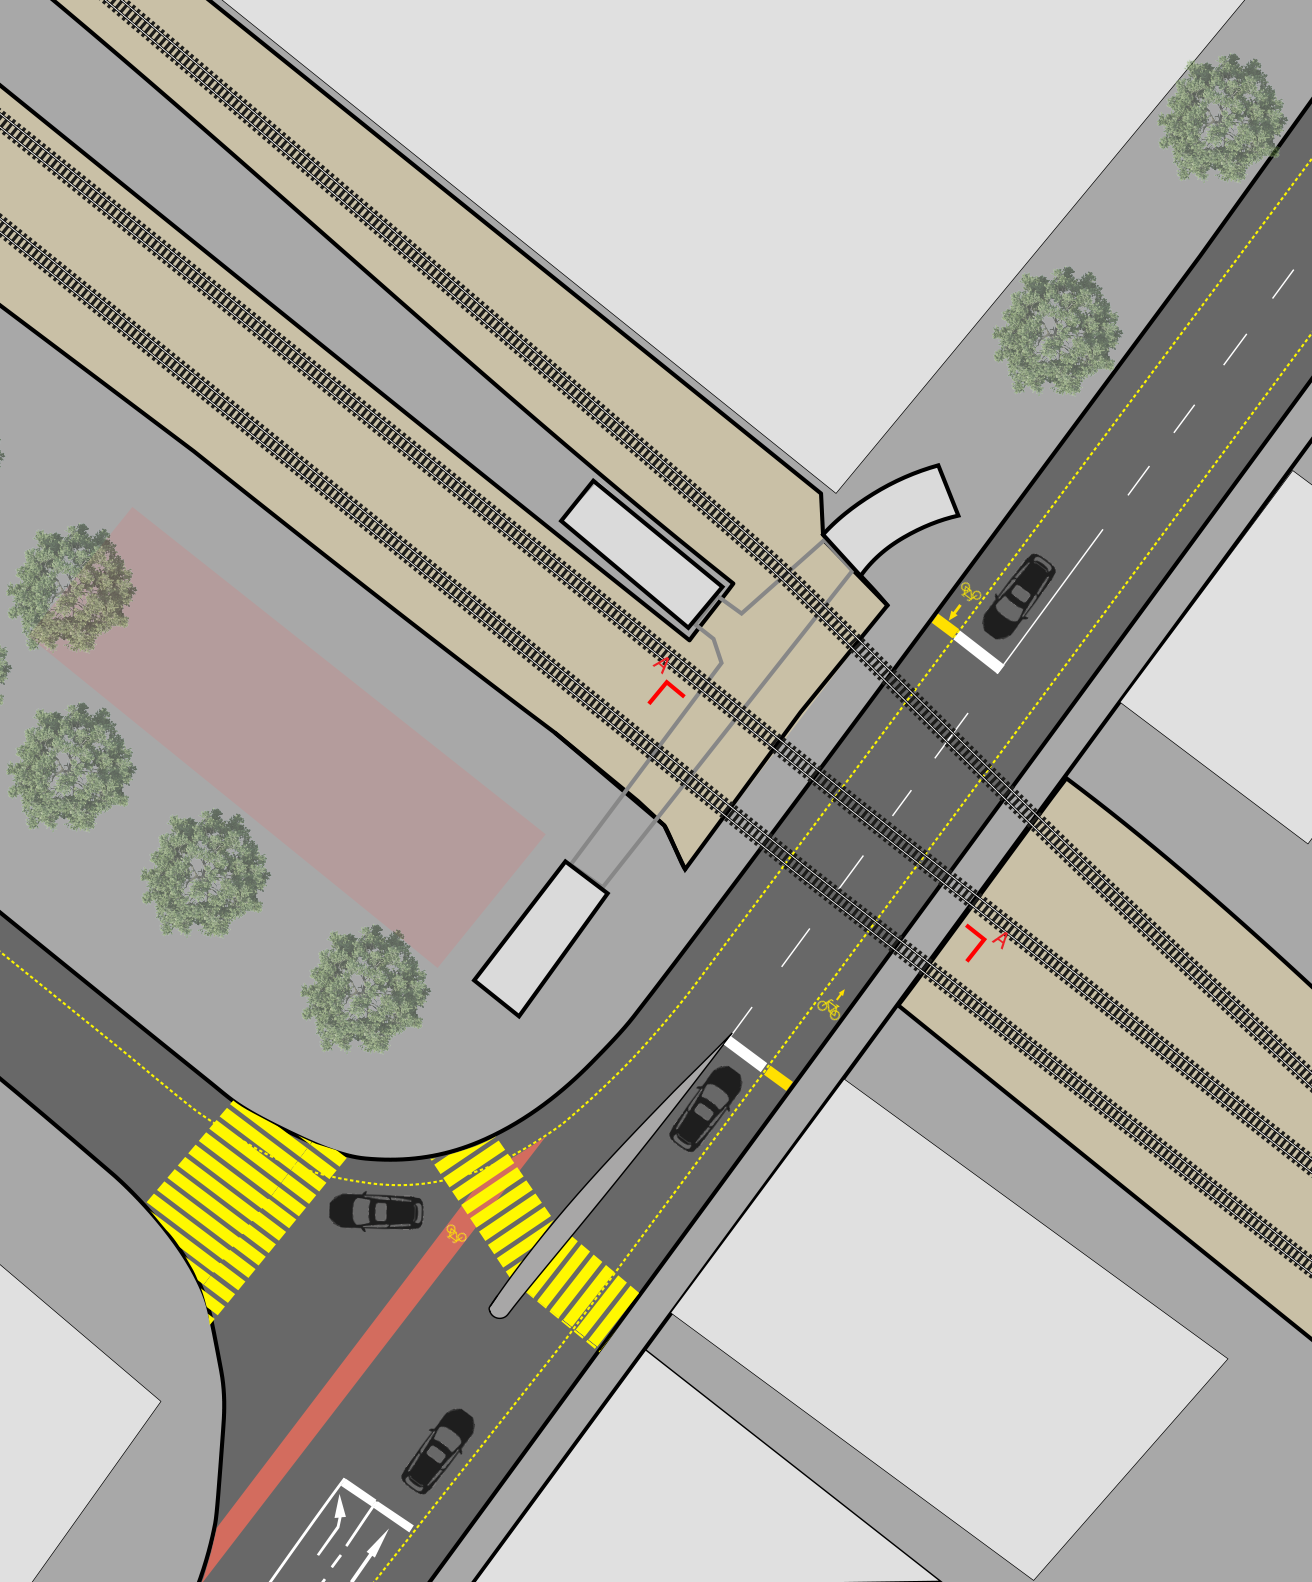
\includegraphics[width=0.65\textwidth]{figures/f-04-05-01-a-V1}
	\caption[Übersicht Variante 1]{Übersicht der Variante 1}
	\label{img:V1Ü}
\end{figure}

\pagebreak

Um die Verkehrssicherheit der Langsamverkehrsteilnehmer minimal zu erhöhen, ist die Anbringung zweier Velostreifen à je 1.5 Meter Breite geplant. Die angenommene maximale Kapazität der beiden Velostreifen zusammen beträgt 3350 Velos pro Stunde. \\
Die Anbringung der Velostreifen erfordert eine geringfügige Verjüngung der Fahrbahn von 4 auf 3.5 Meter pro Fahrbahn. Trotz Verjüngung wird angenommen, dass der zweispurige Strassenabschnitt (eine pro Richtung) eine Kapazität von 2'500 Fahrzeugen pro Stunde aufweist, bei einer geplanten, zulässigen Höchstgeschwindigkeit 50 $km/h$. Unter Berücksichtigung der Situation vor Ort wird angenommen, dass die durchschnittlich gefahrene Geschwindigkeit des MIV 37 $km/h$ beträgt und die der Velofahrer durchschnittlich 15 $km/h$. \\ (\cite{Nacto2018}) (\cite{Mikrozensus2015})

\begin{figure}[h!]
	\centering
	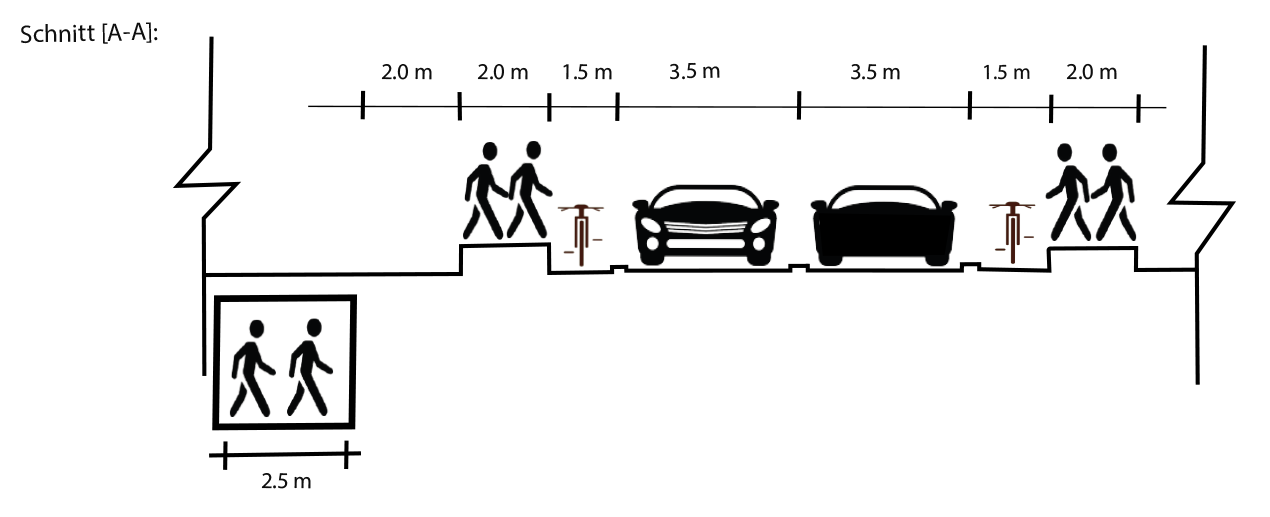
\includegraphics[width=0.7\textwidth]{figures/f-04-05-01-b-V1}
	\caption[Querschnitt Variante 1]{Querschnitt im Schnitt A-A der Variante 1}
	\label{img:V1Q}
\end{figure}

Die Erstellung zweier neuer Radstreifen à je 1.5 Meter Breite kostet gemäss Abschnitt \ref{sub:Unterhalt} 850 CHF pro Laufmeter. Bei einer Gesamtlänge von 80 Meter ergibt sich für den Bau der Variante 1 Kosten im Bereich von 68'000 CHF. (\cite{Baukosten2010}) 

\pagebreak

\subsection{Variante: \ 2}
\label{subsec:V2}
	
Die zweite Variante beinhaltet, wie in Abbildung \ref{img:V2Ü} ersichtlich, den Bau von zwei Velounterführungen, um die lange Wartezeit am Bahnübergang zu verkürzen. Für die Velofahrer entsteht in dieser Variante demnach nur der Zeitverlust gemäss Abschnitt \ref{sub:Reisezeit}, der aufgrund des Befahrens der Infrastruktur entsteht. Die für den MIV angesetzte durchschnittliche Wartezeit beträgt weiterhin 5'. 

Infolge der Rückklassierung der Brunnenstrasse wird ein Tempo 30 Regime eingeführt. Die angenommene durchschnittlich gefahrene Geschwindigkeit des MIV beträgt somit 30 $km/h$ und für die Velofahrer wird angenommen, dass sie mit durchschnittlich 20 $km/h$ durch die Unterführung fahren können. \\ (\cite{Mikrozensus2015})

%\begin{figure}[h!]
 % \centering
 % \subfloat[][]{\label{img:V2Ü}\includegraphics[width=.6\textwidth]{./figures/2}}
  %\hfill
 % \subfloat[][]{\label{img:V2Q}\includegraphics[width=.4\textwidth]{./figures/2_2}}
%\caption[Variante 2]{Übersicht und Querschnitt der Variante 2}
  %\label{fig:V2}
%\end{figure}

\begin{figure}[h!]
	\centering
	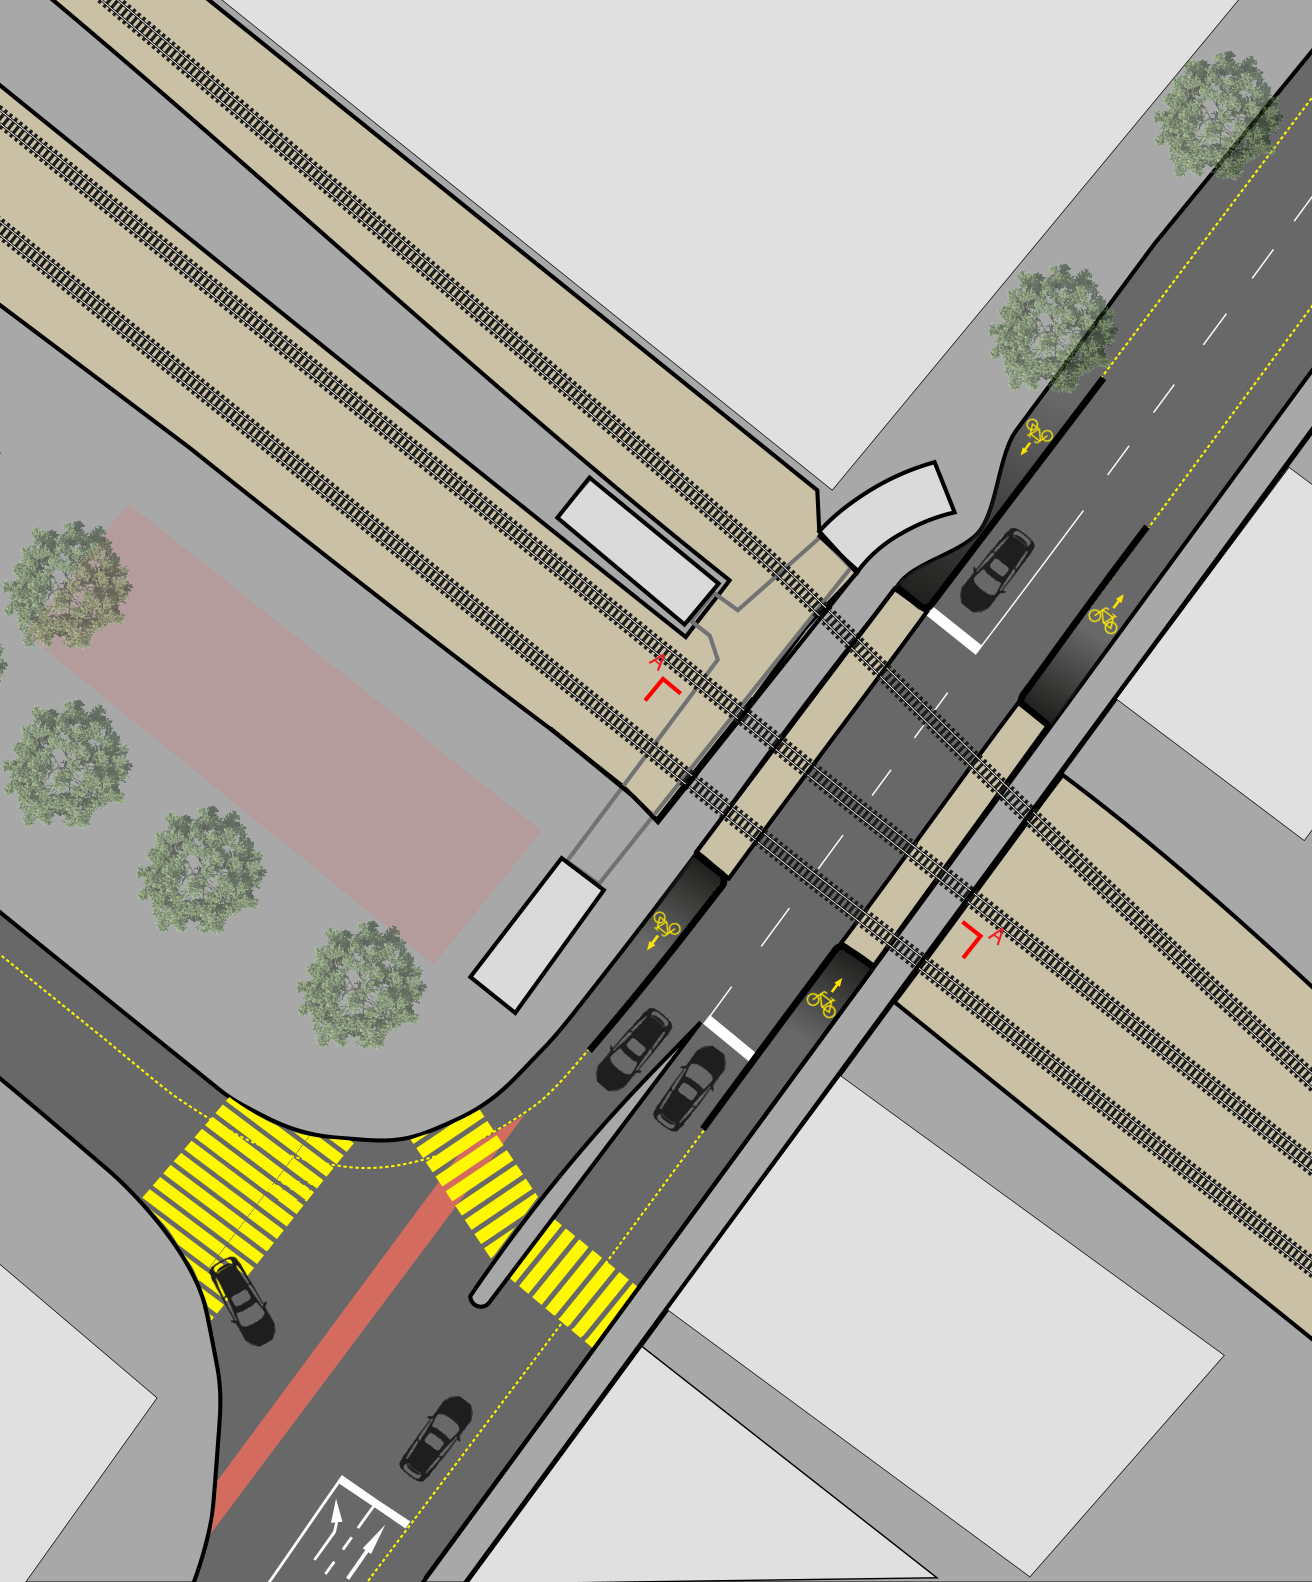
\includegraphics[width=0.65\textwidth]{figures/f-04-05-02-a-V2}
	\caption[Übersicht Variante 2]{Übersicht der Variante 2}
	\label{img:V2Ü}
\end{figure}

Durch den Bau der beidseitig mit einer lichten Breite von 1.5 Meter ausgeführten Velounterführungen, wird einerseits die Verkehrssicherheit der Velofahrer verbessert und andererseits die Kapazität der gesamten Veloinfrastruktur auf maximal 3767 Velos pro Stunde erhöht. Die Gesamtlänge einer Unterführung beträgt in dieser Variante 55 Meter. 
Um diese Unterführung bauen zu können, ist eine weitere Verjüngung der Fahrbahn auf 3 Meter erforderlich, was jedoch zu keiner Reduktion der Kapazität des MIV führen wird.  \\ (\cite{Nacto2018})

\begin{figure}[h!]
	\centering
	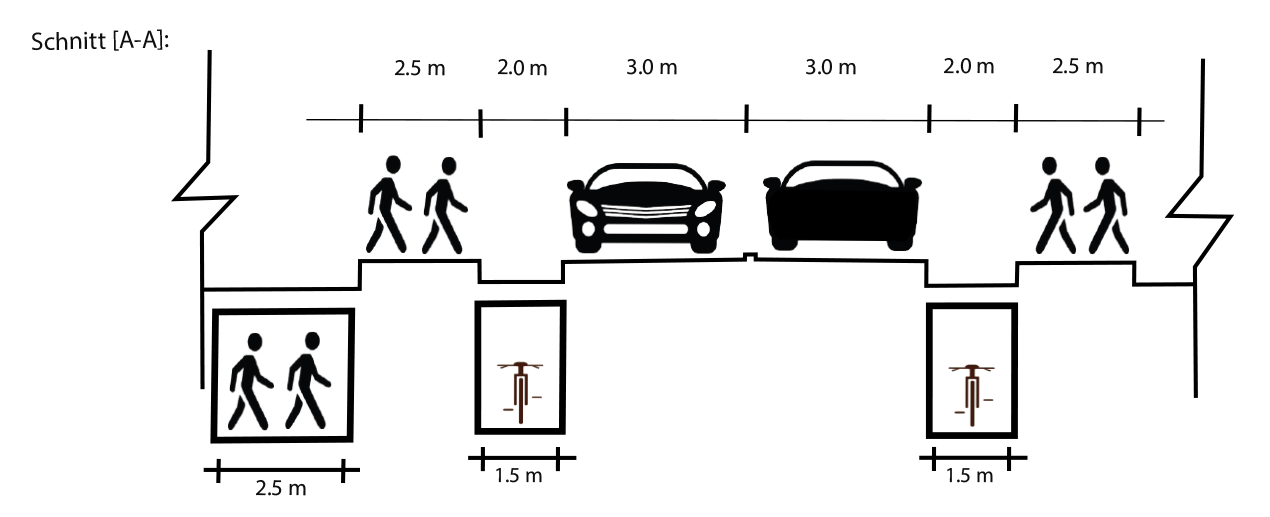
\includegraphics[width=0.7\textwidth]{figures/f-04-05-02-b-V2}
	\caption[Querschnitt Variante 2]{Querschnitt im Schnitt A-A der Variante 2}
	\label{img:V2Q}
\end{figure}

Die prognostizierten Baukosten der Variante 2 werden mithilfe der in Abschnitt \ref{sub:Unterhalt} erläuterten Einheitskosten für den Bau einer Velounterführung und den vorgängig erwähnten Abmessungen der Unterführungen berechnet. Die zu erwartenden Baukosten belaufen sich auf 1.16 Mio. CHF, wobei 520'000 CHF für die vier Rampen und 640'000 CHF für den Bau der Unterführungen unter dem Lastfall Eisenbahn sowie das Anbringen der Velostreifen anfallen. (\cite{Baukosten2010}) 

\pagebreak

\subsection{Variante: \ 3}
\label{subsec:V3}

Die dritte Variante habe ich ausgehend von der Variante 2 entwickelt und ist ein Versuch die Verkehrssicherheit sowie den Fahrkomfort für die Velofahrer zu steigern. Um dies zu erreichen, wird, wie in Abbildung \ref{img:V3Ü} ersichtlich, die Velounterführung zweispurig ausgeführt, was zur Folge hat, dass die Strasse einspurig über den Bahnübergang geführt werden muss. Diese Strassenführung erfordert die Einführung eines Ampelsystems, was die durchschnittliche Wartezeit für den MIV, bei einem Rotlichtzyklus von einer Minute, auf 7 Minuten erhöht. Für das Ampelsystem wäre zusätzlich eine Busbevorzugungsanlage zu prüfen. \\

Die maximale Höchstgeschwindigkeit beträgt wie in Variante 2 30 $km/h$, wobei angenommen wird, dass die Velofahrer mit bis zu 30 $km/h$ durch die Unterführung fahren könnten. (\cite{Mikrozensus2015})

%\begin{figure}[h!]
 % \centering
  %\subfloat[][]{\label{img:V3Ü}\includegraphics[width=.6\textwidth]{./figures/3}}
  %\hfill
 % \subfloat[][]{\label{img:V3Q}\includegraphics[width=.4\textwidth]{./figures/3_2}}
%\caption[Variante 3]{Übersicht und Querschnitt der Variante 3}
 % \label{fig:V3}
%\end{figure}

\begin{figure}[h!]
	\centering
	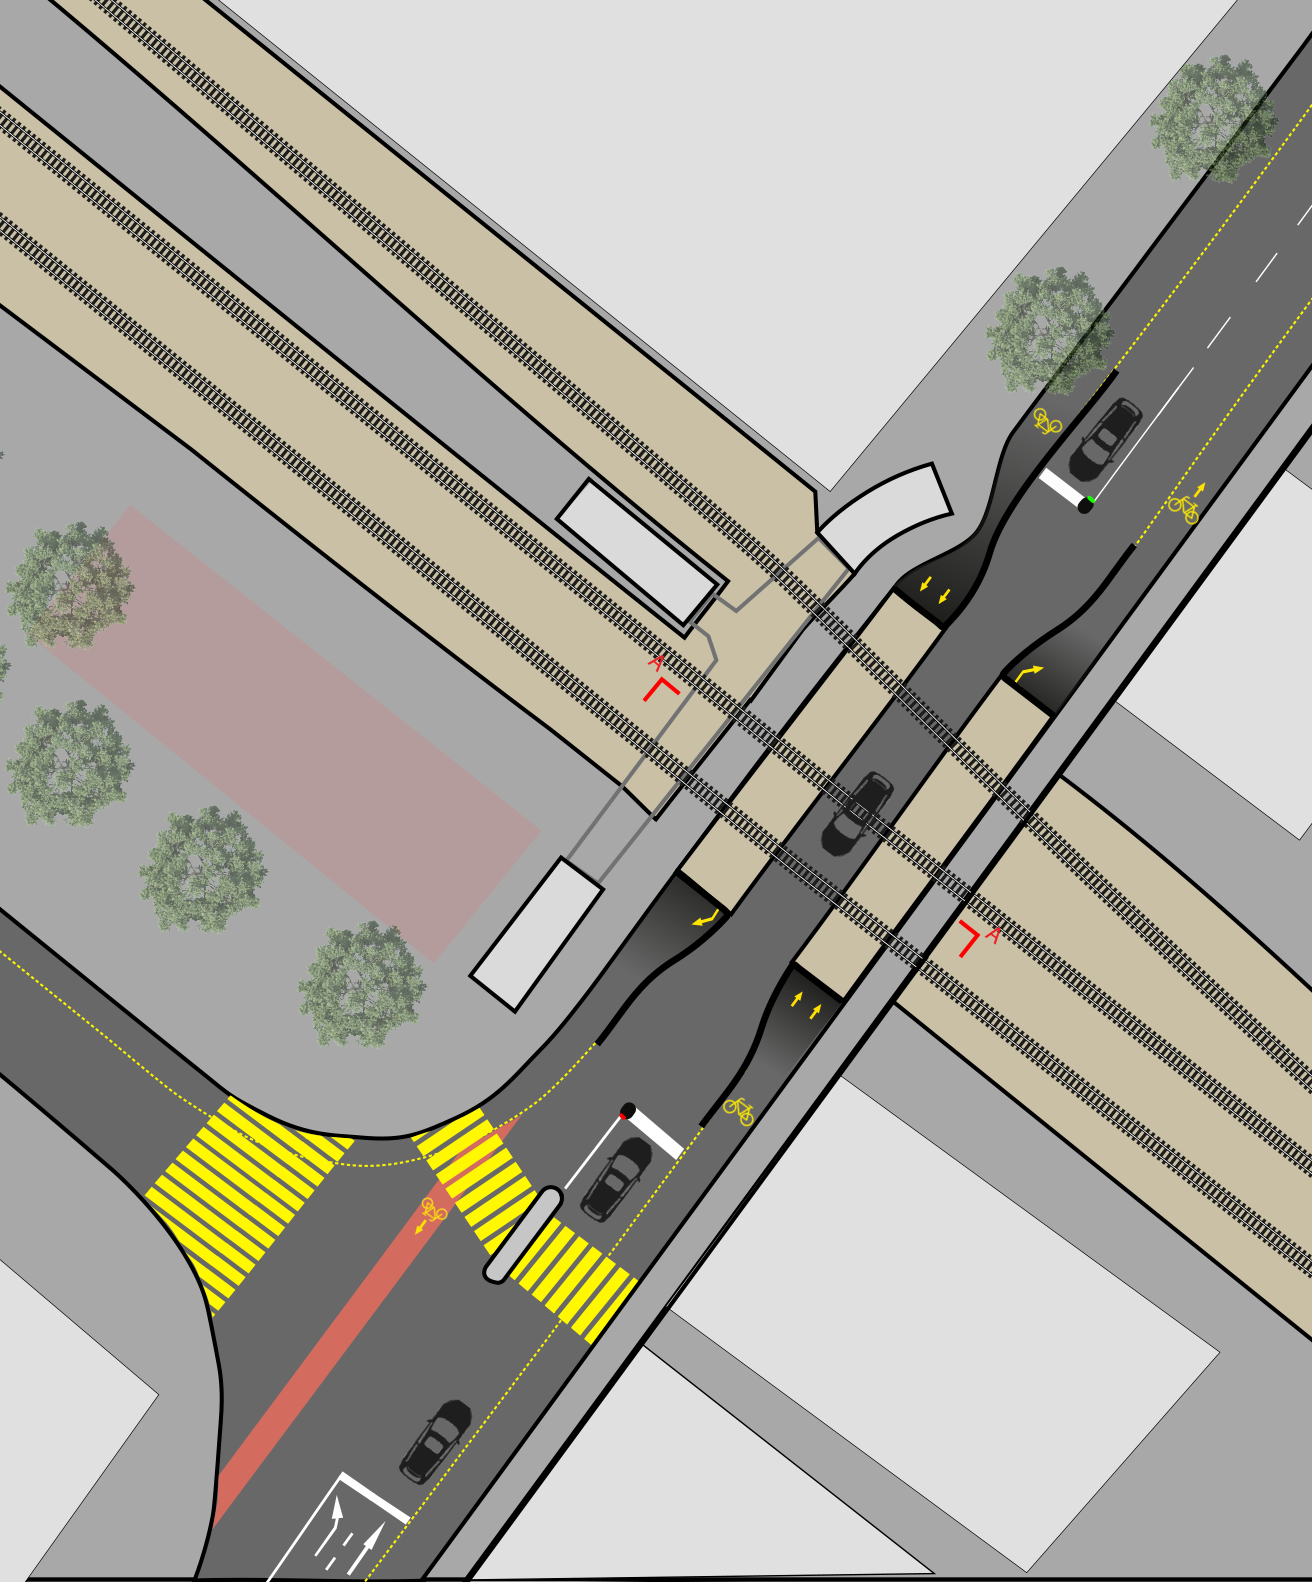
\includegraphics[width=0.65\textwidth]{figures/f-04-05-03-a-V3}
	\caption[Übersicht Variante 3]{Übersicht der Variante 3}
	\label{img:V3Ü}
\end{figure}

Die lichte Breite der Velounterführung beträgt 2 Meter und die Gesamtlänge einer Unterführung beläuft sich auf 65 Meter. Die zweispurige Strassenführung wird mit Fahrbahnmarkierungen verdeutlicht. Es wird angenommen, dass durch diese Ausführung die Kapazität der gesamten Veloinfrastruktur auf maximal 4600 Velos pro Stunde erhöht wird. \\(\cite{Nacto2018})

Infolge der Reduktion der Strasseninfrastruktur um eine Spur nehme ich, dass sich die Kapazität auf 1'250 Fahrzeuge pro Stunde halbiert. Die Fahrspur bleibt mit 5 Meter für grosse Busse weiterhin problemlos befahrbar.

\begin{figure}[h!]
	\centering
	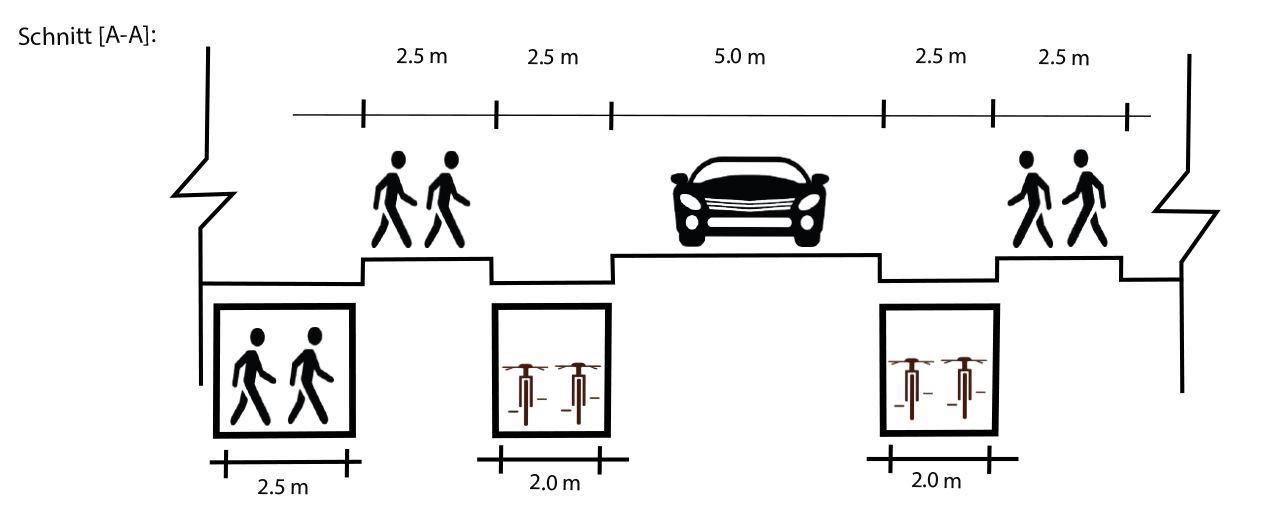
\includegraphics[width=0.7\textwidth]{figures/f-04-05-03-b-V3}
	\caption[Querschnitt Variante 3]{Querschnitt im Schnitt A-A der Variante 3}
	\label{img:V3Q}
\end{figure}

Die Baukosten der Variante 3 belaufen sich auf insgesamt 1.51 Mio. CHF und werden wie für Variante 2 berechnet. Für den Bau der Unterführung unter dem Lastfall Eisenbahn und das Anbringen der Velostreifen sind 988'000 CHF vorgesehen und für den Bau der vier Rampen fallen 520'000 CHF an. \\ (\cite{Baukosten2010}) 


In Tabelle \ref{tab:t-08-01-Varianten} werden die, für die Berechnung der Kosten verwendeten Eigenschaften der Varianten zusammengefasst.
%=============================================================================
% Thesis Template in LaTex
%
% File:  t-05-01-IsingModel.tex -- Table for the Ising
% Author(s): Juergen Hackl <hackl@ibi.baug.ethz.ch>
%            Clemens Kielhauser <kielhauser@ibi.baug.ethz.ch>
%
% Creation:  27 Jan 2014
% Time-stamp: <Tue 2013-08-13 20:14 juergen>
%
% Copyright (c) 2014 Infrastructure Management Group (IMG)
%               http://ibi.ethz.ch
%
% More information on LaTeX: http://www.latex-project.org/
%=============================================================================
%\small\renewcommand{\arraystretch}{1.2} 
%


\begin{table}[h!]
\scriptsize
{\setstretch{0.6}
%\renewcommand{\arraystretch}{1.4}
\flushleft
\begin{tabular}{@{}p{5cm} p{2.5cm} p{2.5cm} p{2.5cm}@{}} \\   
\toprule 		
\textbf{Eigenschaften}  				   								&\textbf{Variante\,1}  & \textbf{Variante\,2} & \textbf{Variante\,3}   \\			
\midrule 
Länge Fahrbahn ($m$)         	 		   								& 80                    & 80    			   & 80             	\\
Länge Unterführung ($m$)       	 		   								& -                     & 55    			   & 65             	\\
Velospuren:					   											&  2				    &  2				   &  4         		\\
Fahrbahnen									 		   					&  2				    &  2				   &  1         		\vspace*{0.25mm} \\
Breite eines Veloweg ($m$):				   								&  1.5				    &  1.5				   &  2         		\\
Breite einer Fahrbahn ($m$):			 		   					    &  3.5				    &  3				   &  5         		\vspace*{0.25mm} \\
Tempolimit	($\frac{km}{h}$) 		   						    		& 50				    & 30				   & 30                	\\
\underline{$\varnothing$\,Geschwindigkeit} ($\frac{km}{h}$) 			&       	            &   				   &               		 \\
\hspace*{5mm}\textbullet\, Velo            		       					& 15  					& 20    			   & 25      			\\
\hspace*{5mm}\textbullet\, MIV            		       					& 37  					& 30    			   & 30      			\vspace*{0.25mm} \\
\underline{Kapazität} ($\frac{Fahrzeug}{h}$)		        			&    				    &  				       &                  	 \\
\hspace*{5mm}\textbullet\, Velo            	       					    & 3350 					& 3767    			   & 4600      			\\
\hspace*{5mm}\textbullet\, MIV         		       					    & 2500 					& 2500    			   & 1250      			\\
\underline{Wartezeit} ($Minuten$)        		    			   		&    				    &  				       &                  	 \\
\hspace*{5mm}\textbullet\, Velo            	       					    & 5 					& 5    			       & 7      			\\
\hspace*{5mm}\textbullet\, MIV         		       					    & 5  					& 0      			   & 0      			\\
Baukosten ($CHF$)														& 68'000				& 1.16 Mio.			   & 1.51 Mio.           \\
\bottomrule

\end{tabular}
\caption{Basis Informationen der Varianten}
\label{tab:t-08-01-Varianten}
}
\end{table}


%=============================================================================
% EOF
%

%%% Local Variables:
%%% mode: latex
%%% TeX-master: "../guidelines"
%%% End:



\pagebreak

% ===========================================================================
% EOF
%

%%% Local Variables:
%%% mode: latex
%%% TeX-master: "../main"
%%% End:


%----------------------

\section{Analyse der Lösungen}
\label{sec:Analyse}

Um den Vergleich der Varianten, zur Bestimmung der optimalen Lösungen, durchführen zu könne, müssen die Kosten anhand der unter Abschnitt \ref{sec:Kostenstruktur} dargestellten Formeln, berechnet werden. Um die Kosten über einen Zeitraum von vierzig Jahren berechnen zu könne, muss der Einfluss der unter Abschnitt \ref{subsec:Uncertain} bestimmten Faktoren, auf das DTV modelliert werden und somit der DTV für die Zukunft geschätzt werden. Dies geschieht anhand der nachfolgend vorgestellten Szenarien.


	\subsection{Modellierung des DTV}
	\label{subsec:Modellierung}
	
Die Zentrumsentwicklung, die Aufwertung der Quartiere nördlich des Bahnhofs, die Massnahmen zur Verkehrsberuhigung, der Ausbau der Veloparkieranlagen am Bahnhof sowie der Ausbau des Spitals und die im Rahmen der Umsetzung des Leitziels "Uster steigt um!" getroffenen Massnahmen zur Förderung des Langsamverkehrs, haben direkt oder indirekt einen Einfluss auf den Langsamverkehr am Bahnübergang. Unter anbetracht der Tatsache, dass alle diese genannten Einflussfaktoren auf die Verkehrssituation am Bahnübergang, zu mehr Veloverkehr führen werden, fasse ich diese unter dem Stichpunkt \textit{Umsetzung des STEK} zusammen und modelliere sie, mit den in Abschnitt \ref{subsubsec:Umsetzung} vorgestellten Szenarien. Da das Bevölkerungswachstum den grössten Effekt auf das DTV haben wird, untersuche ich diese Einfluss anhand der im Abschnitt \ref{subsubsec:Bevölkerung} dargestellten Szenarien, separat. 

Die zukünftige Situation am Bahnübergang wird somit sowohl durch die Bevölkerungsentwicklung als auch durch die Umsetzun des STEK beeinflusst. Diese Einflüsse tretten gleichzeitig auf, was dazu führt, dass, um die Berechnung der Kosten der Varianten unter Berücksichtigung der unsicheren zukünftigen Entwicklung der Einflussfaktoren durchführen zukönnen, eine Kombination der entwickelten Szenarien betrachtet werden muss. Eine solche Kombination stellt ein mögliches zukünftiges Ereigniss dar. 

\begin{figure}[h!]
	\centering
	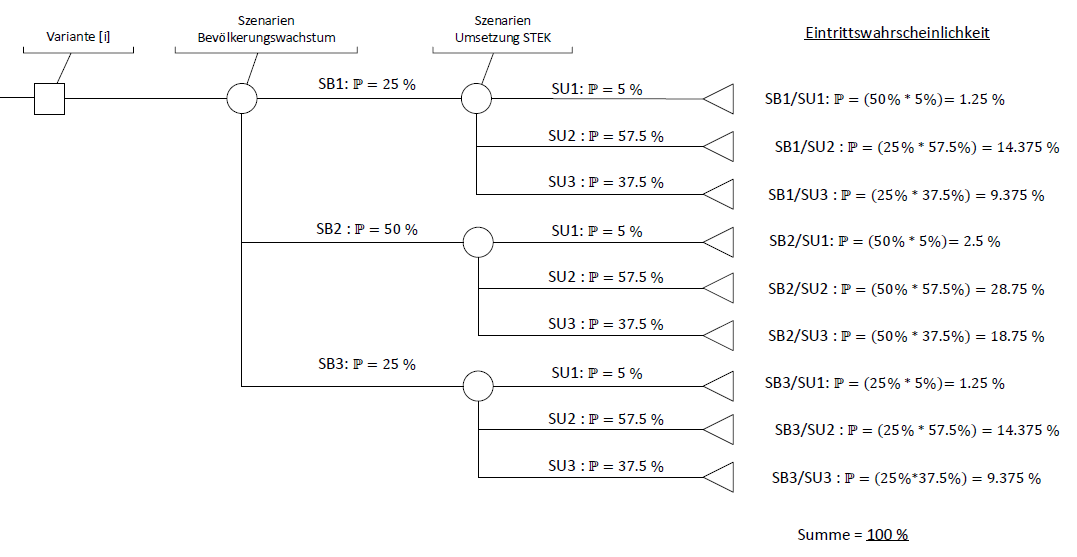
\includegraphics[width=\textwidth]{figures/f-04-06-01-Entscheidungsbaum-Szenarien}
	\caption[Szenarienübersicht]{Übersicht über die Szenarien und ihre Eintrittswahrscheinlichkeiten}
	\label{img:EntscheidunSzenarien}
\end{figure}

Eine Vorhersage über die Zukunft zumachen, ist nur mit einer gewissen Unsicherheit möglich. Um diese Unsicherheit in die Optimierung mitein beziehen zu können, bewerte ich das Eintretten dieser Szenarien mit einer Wahrscheinlichkeit $[0,1]$, der sogenannte Eintrittswahrscheinlichkeit eines Szenarios.
Die Eintrittswahrscheinlichkeit eines kombinierten Szenarios, sprich eines zukünftigen Ereigniss, berechnet sich wie in Abbildung \ref{img:EntscheidunSzenarien} dargestellt aus der Multiplikation der Eintrittswahrscheinlichkeiten der Ausgangsszenarien.
Dies stellt zugleich ein Ausschnit aus dem Entscheidungprozess zur Bestimmung der optimalen Lösung dar.

\pagebreak

	%=============================================================================
% Thesis Template in LaTex
%
% File:  04-06-Szenarien.tex -- Fallstudie/Modellierung der ungewissen Parameter
% Author(s): Jürgen Hackl <hackl@ibi.baug.ethz.ch>
%            Clemens Kielhauser <kielhauser@ibi.baug.ethz.ch>
%
% Creation:  27 Jan 2014
% Time-stamp: <Tue 2013-08-13 20:14 juergen>
%
% Copyright (c) 2014 Infrastructure Management Group (IMG)
%               http://ibi.ethz.ch
%
% More information on LaTeX: http://www.latex-project.org/
%=============================================================================

% Unterkapitel Szenarien
% ---------

\subsubsection*{Bevölkerungswachstum}
\label{subsubsec:Bevölkerung}

Wie in Kapitel \ref{chap:Fallstudie} erwähnt, ist das DTV mehrheitlich von der zukünftigen demographischen Entwicklung abhängig.
Um den Effekt, den das Bevölkerungswachstum auf das DTV haben wird, modellieren zu können, orientiere ich mich an den Wachstumsprognosen der Stadt Uster.
Die zu erwartende Bevölkerungsentwicklung habe ich dem Kapitel 3 \textit{Stadt Uster im Porträt} des STEK entnommen und wird nachfolgend kurz beschrieben. 

\begin{description}
\item[Stagnation] \hfill \\
Geschätzte Anzahl an Einwohner im Jahr 2035: 38'760 \\
$\Rightarrow$ + 188 Einwohner/Jahr \\ $\Rightarrow$ + 0.5\% pro Jahr gegenüber 2015
\item[Trend restriktiv] \hfill \\
Geschätzte Anzahl an Einwohner im Jahr 2035: 42'260 \\ 
$\Rightarrow$ + 363 Einwohner/Jahr \\ $\Rightarrow$ + 1\% pro Jahr gegenüber 2015
\item[Trend Prosperität] \hfill \\
Geschätzte Anzahl an Einwohner im Jahr 2035: 45'620 \\ 
$\Rightarrow$+ 531 Einwohner/Jahr \\ $\Rightarrow$ + 1.5\% pro Jahr gegenüber 2015
\end{description}

Anhand dieser Wachstumsprognosen und unter der Annahme eines linearen Wachstums, definiere ich die drei nachfolgend dargestellten Szenarien. Mit diesen Szenarien werde ich in einem nächsten Schritt den zukünftigen DTV für den MIV und den Langsamverkehr, sprich Veloverkehr, am Bahnübergang Brunnenstrasse ermitteln.
Ausgehend vom DTV des MIV im Jahr 2016 und den Wachstumsraten der Szenarien habe ich die jährliche Zunahme an Motorfahrzeugen ermittelt. Im Jahr 2016 lag das DTV des MIV am Bahnübergang bei 12'023 Motorfahrzeugen pro Tag. \\ (\cite{GIS})

\begin{itemize}
\item Szenario: SB 1
	\begin{itemize}
	\item Grundlage: Stagnation $\Rightarrow$ jährliches Wachstum um 0.5\%
	\item Jährliche Zunahme DTV: 60 Fahrzeuge
	\item Eintrittswahrscheinlichkeit: 25\%
	\end{itemize}
\item Szenario: SB 2
	\begin{itemize}
	\item Grundlage: Trend restriktiv  $\Rightarrow$ jährliches Wachstum um 1 \%
	\item Jährliche Zunahme DTV: 120 Fahrzeuge
	\item Eintrittswahrscheinlichkeit: 50\%
	\end{itemize}
\item Szenario: SB 3
	\begin{itemize}
	\item Grundlage: Trend Prosperität  $\Rightarrow$ jährliches Wachstum um 1.5\%
	\item Jährliche Zunahme DTV: 180 Fahrzeuge
	\item Eintrittswahrscheinlichkeit: 25\%
	\end{itemize}
\end{itemize}


Die Wahrscheinlichkeit das Szenario SB 2 eintritt und das DTV jährlich um 120 Fahrzeuge zunimmt, bewerte ich mit 50\%. Dies erfolgt unter der Annahme, dass der restriktive Trend das minimale Wachstumsziel von 20\% wiederspiegelt, welches gemäss dem STEK mit grösster Wahrscheinlichkeit eintreten wird, und da dieses Szenario den kantonalen Prognosen entspricht, erachte ich dieses Szenario als das wahrscheinlichste und bewerte es dementsprechend.

Das es zu einem verstärktem Wachstum von 1.5\% und somit zu einer jährlichen Zunahme von 180 Fahrzeugen am DTV kommt, erachte ich nach den Angaben des STEK als unwahrscheinlich, da ein übermässiges Bevölkerungswachstum aufgrund der nur beschränkt vorhandenen Kapazitäten zur Erweiterung der Wohnangebots, nur bedingt möglich ist. 

Das es zu einer Stagnation des Bevölkerungswachstums und im Zuge dieser Modellierung zu einem Verkehrswachstum von 0.5\% und einer jährlichen Zunahme von 60 Fahrzeugen am DTV kommt, erachte ich in Anbetracht der Prognosen zur demographische Entwicklung im Kanton Zürich, als unwahrscheinlich. Deshalb bewerte ich die Szenarien SB 1 und SB 3 mit jeweils 25\%.

Mithilfe der verschiedenen Wachstumsraten $WR_{s}$ der Szenarien und der Formel \ref{eq.11} berechne ich das $DTV_{i}$ im Jahr $t_{i}$. \\
Der DTV des Jahres 2016 lag, wie oben erwähnt, bei 12'023 Motorfahrzeuge pro Tag. Diesen Wert nutze ich als Start- sowie Basiswert meiner Berechnungen. 

\begin{equation}
DTV_{i} = DTV_{2016} + \bigl( t_{i} - t_{2016} \bigr) \cdot \bigl[WR_{s}\bigr] \cdot DTV_{2016}
\label{eq.11}
\end{equation}

Da die Anzahl Velos, die den Bahnübergang Brunnenstrasse täglich passieren, nicht von einer Verkehrsmessstelle gezählt werden, muss diese Information aus dem MIV hergeleitet werden. Dies erfolgt mithilfe der Daten der Verkehrsmessstelle an der etwas südlich von Uster gelegenen Seefeldstrasse, welche Niederuster mit Riedikon verbindet. 
Der im Jahr 2019 gemessen durchschnittliche DTV lag bei 8818 Motorfahrzeugen für das MIV und 913 Velos. Daraus ergibt sich einen Veloanteil von 10.35\%. \footcite{MIVSeefeld}\footcite{VeloSeefeld}

\begin{align*}
\mu &= \frac{DTV_{Velo,Seefeldstrasse}}{DTV_{MIV,Seefeldstrasse}}   \\[2ex]
DTV_{Velo} &= DTV_{MIV} \cdot \mu_{Velo} 
\end{align*}

In den Abbildung \ref{fig:DTV} sind die Ergebnisse meiner Modellierung des DTV am Bahnübergang Brunnenstrasse dargestellt, die ich für die Berechnung der Kosten der Varianten verwenden werde. Eine ausführliche Tabelle aller modellierten DTV-Werte findet sich unter Abschnitt \ref{subsec:DTVModellierung}

\begin{figure}[h!]
  \centering
  \subfloat[][]{\label{fig:04-06-02-DTV(MIV)}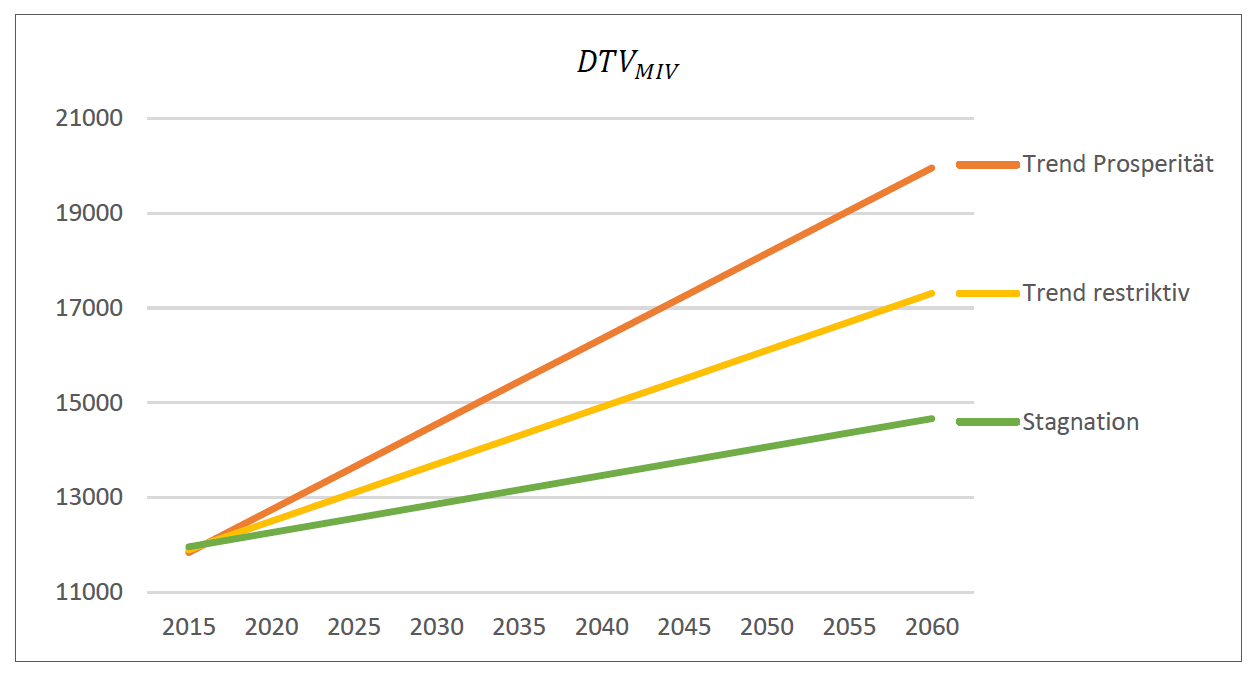
\includegraphics[width=.5\textwidth]{./figures/f-04-06-02-DTV(MIV)-SzenarienBev-Wachstum}}
  \hfill
  \subfloat[][]{\label{fig:04-06-03-DTV(VELO)}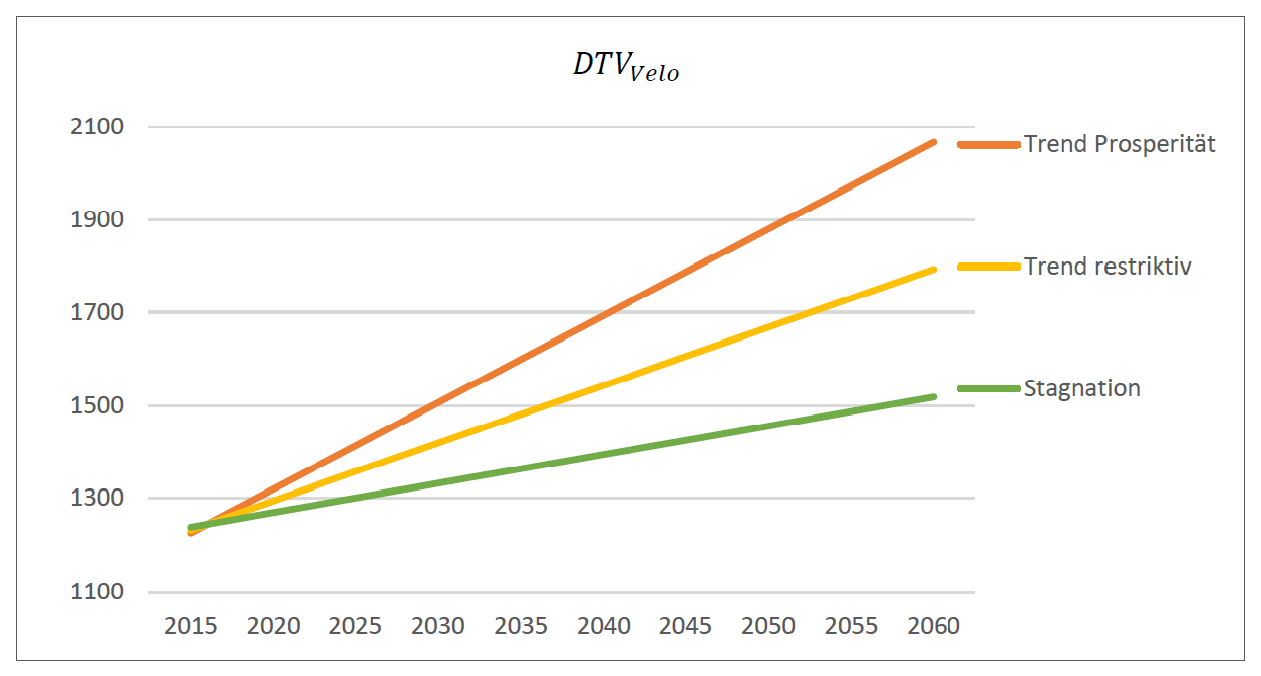
\includegraphics[width=.5\textwidth]{./figures/f-04-06-03-DTV(VELO)-SzenarienBev-wachstum}}
\caption[DTV Brunnenstrasse]{DTV an der Brunnenstrasse}
  \label{fig:DTV}
\end{figure}



\subsubsection*{Umsetzung STEK}
\label{subsubsec:Umsetzung}

Die folgenden Szenarien modellieren die Effekte, den die in Abschnitt \ref{subsec:Modellierung} unter dem Stickwort \textit{Umsetzung STEK} zusammengefassten Einflussfaktoren, auf den $DTV_{Velo}$ haben werden. 

Das meines Erachtens mit grösster Wahrscheinlichkeit eintretende Szenario entspricht der Verkehrsprognose des Bundes, die eine Zunahme der Verkehrsleistung des Langsamverkehrs bis 2040 gegenüber 2010, um 32\% erwartet. (\cite{Perspektive2040}) 

Um die Ober- sowie Untergrenze meiner Prognose ermitteln zu können, orientiere ich mich ein weiteres Mal am STEK. Mithilfe der unter Kapitel 10 \textit{Stadt Uster im Porträt} des STEK vorgestellten Wachstumsprognosen für die Bevölkerungsentwicklung sowie der in Kapitel 7 \textit{Mobilität} des STEK gemäss regionalem Richtplan erstellten Verkehrsprognose für den Anteil der Velofahrer am Gesamtverkehr, erstelle ich zwei weitere Szenarien. 
Einerseits berücksichtige ich den Fall einer ungenügenden Umsetzung der Leitziele und der daraus resultierenden stagnierenden Entwicklung des Veloverkehrs. Andererseits den Fall einer maximalen Umsetzung aller Ziele in Verbindung mit einer Verschiebung des Innerstädtischen Modalsplit in Richtung Langsamverkehr.

\pagebreak

\begin{description}
\item[Stagnation] \hfill \\
Prognose gemäss STEK: $\Rightarrow$ jährliches Wachstum: 0.54 \% 
\item[Verkehrsperspektiven 2040] \hfill \\
Prognostizierte Zunahme der Verkehrsleistung: 32\% $\Rightarrow$ jährliches Wachstum: 1.3 
\item[Umsetzung maximal] \hfill \\
Prognose gemäss STEK und regionalem Richtplan: $\Rightarrow$ jährliches Wachstum: 2 \% 
\end{description}

Eine Stagnation erachte ich unter Berücksichtigung der Entwicklung des Langsamverkehrs über die letzten zehn Jahre, als unwahrscheinlich und bewerte das Eintreten dieser Prognose demzufolge mit 5\%. \\
Dass es zu einem Wachstum gemäss der Prognose des Bundes kommen wird, erachte ich nach der Konsultation weitere Verkehrsprognosen, als das Szenario, welches mit grösster Wahrscheinlichkeit eintreten wird. Daher bewerte ich dieses Szenario mit einer Eintrittswahrscheinlichkeit von 57.5\%. \\
Dass alle Ziele maximal erfüllt werden und eine Verschiebung des innerstädtischen Modal-Split stattfindet, erachte ich mit 32.5\% als deutlich plausibler als die Stagnation, jedoch als unwahrscheinlicher als die Prognose des Bundes. 

\begin{itemize}
\item Szenario: SU 1
	\begin{itemize}
	\item Grundlage: Stagnation 
	\item Eintrittswahrscheinlichkeit: 5\%
	\end{itemize}
\item Szenario: SB 2
	\begin{itemize}
	\item Grundlage: Verkehrsperspektiven 2040
	\item Eintrittswahrscheinlichkeit: 57.5\%
	\end{itemize}
\item Szenario: SB 3
	\begin{itemize}
	\item Grundlage: Umsetzung maximal
	\item Eintrittswahrscheinlichkeit: 32.5\%
	\end{itemize}
\end{itemize}

Anhand der zu Beginn dieses Abschnitts definierten Wachstumsraten, sowie ausgehend von den Messwerten des täglichen Veloverkehrs im Jahr 2016, habe ich die Anzahl Velos, die in jedem Szenario zusätzlich pro Tag auf der Infrastruktur unterwegs sein werden, ermittelt. 
Die Anzahl Velos die im Jahr 2016 täglich den Bahnübergang nutzten, lag, gemäss Abschnitt \ref{subsubsec:Bevölkerung}, bei 1245.

Das Szenario SU 1 führt somit zu einer Erhöhung des täglichen Veloverkehrs um 7 Velos pro Jahr, das Szenario SU 2 zu einer Zunahme von 16 Velos pro Jahr und das Szenario SB 3 zu einer Erhöhung des $DTV_{Velo}$ um 25 Velos pro Jahr. 
Mit diesen Angaben berechne ich die Anzahl Velos, die je nach Szenario, zusätzlich zu den in Abschnitt \ref{subsubsec:Bevölkerung} berechneten DTV-Werten, auf der Infrastruktur unterwegs sein werden.

\pagebreak

% ===========================================================================
% EOF
%

%%% Local Variables:
%%% mode: latex
%%% TeX-master: "../main"
%%% End:



	\subsection{Berechnung der Kosten der Varianten}
	\label{subsec:Kostenberechnung}
	%=============================================================================
% Thesis Template in LaTex
%
% File:  04-07-Kosten -- Analyse der Lösungen - Fallstudie
% Author(s): Jürgen Hackl <hackl@ibi.baug.ethz.ch>
%            Clemens Kielhauser <kielhauser@ibi.baug.ethz.ch>
%
% Creation:  27 Jan 2014
% Time-stamp: <Tue 2013-08-13 20:14 juergen>
%
% Copyright (c) 2014 Infrastructure Management Group (IMG)
%               http://ibi.ethz.ch
%
% More information on LaTeX: http://www.latex-project.org/
%=============================================================================

% Unterkapitel Kosten
% ---------

Die Berechnung der Kosten der Varianten erfolgt ahand der Berchnung der Zielfunktion über den Zeitraum von 40 Jahren. In Abbildung \ref , wird für die Variante 1 im Szenario SB1/SU1, die Berechnung der ersten 5 Jahre gezeigt. Zur Übersicht zeige ich die Formel der Zielfunktion hier erneut. 

\begin{equation*}
Min. \thinspace TK_{i} = Min. \thinspace [K_{U}^i + K_{B}^i + K_{TT}^i + K_{E}^i + K_{A}^i]
\end{equation*} 

Was man im Excell sieht:

-> DTV die ich in mit den im vorangegangenen Abschnitt erläuterten Szenarien ermittelt habe.

Mit excell beispiel File... gemäss MA BSP

Was genau mache ich:
-Berechnung der Zielfunktion über den betrachteten Zeithorizont
-Darstellen der Szenarien mit ihren Eintrittswahrscheinlichkeiten
-Kombination der berechneten Kosten mit den Eintrittswahrscheinlichkeiten -> ergibt die Risiken der Varianten
-Summe aller Risiken ergibt das Risiko der Variante selbst.

% ===========================================================================
% EOF
%

%%% Local Variables:
%%% mode: latex
%%% TeX-master: "../main"
%%% End:


%---------------------

\section{Bewertung der Lösungen}
\label{sec:Bewertung}

Da die berechneten Kosten einer Variante in einem Szenario vom jeweiligen Szenario abhängt, muss, um eine von den Szenarien unabhängige Bewertung der Varianten vornehmen zu können, die berechneten Kosten mit den Eintrittswahrscheinlichkeit des jeweiligen Szenarios gewichtete werden. Diese wahrscheinlichkeitsgewichteten Kosten die aufgrund der Ausführung einer Variante in einem der Szenarien entstehen, nenne ich im Rahmen dieser Untersuchung; Risiko. \\
Dies geschieht, um die Unsicherheiten, welche bei der Vorhersage der Wahrscheinlichkeit des Eintrettens der Szenarien entstehen, in die Bewertung der Varianten miteinfliessen zulassen. 

Als letzter Schritt der Bewertung wird mit Hilfe der Sensitivitätsanalysen der rechten Seite der Zielfunktion, die Robustheit der gefundenen optimalen Lösung überprüft sowie die Abhängigkeit von den getroffenen Annahmen aufgezeigt.


	\subsection{Berechnung der Risiken der Varianten}
	%=============================================================================
% Thesis Template in LaTex
%
% File: 04-08-Risiken - Bewertung der Lösung -- Fallstudie
% Author(s): Jürgen Hackl <hackl@ibi.baug.ethz.ch>
%            Clemens Kielhauser <kielhauser@ibi.baug.ethz.ch>
%
% Creation:  27 Jan 2014
% Time-stamp: <Tue 2013-08-13 20:14 juergen>
%
% Copyright (c) 2014 Infrastructure Management Group (IMG)
%               http://ibi.ethz.ch
%
% More information on LaTeX: http://www.latex-project.org/
%=============================================================================

% Unterkapitel Risikenberechnung 
% ---------
\label{subsec:BerechnungRisiken}


Wie im vorangegangen Abschnitt erwähnt, berechnet sich das Risiko einer Varianten in einem Szenario, durch die Multiplikation der Eintrittswahrscheinlichkeit des Szenarios mit den für die jeweilige Variante, im betrachteten Szenario, berechneten Kosten. Das Gesamtrisiko das von der Durchführung einer Variante ausgeht, setzt sich somit aus der Summe aller Risiken einer Variante zusammen. 
Anhand der nachfolgenden Abbildung wird als Beispiel die Berechnung des Risiko der Variante 1, mithilfe eines Entscheidungsbaums gezeigt. Die Berechnung erfolgt in diesem Fall von Rechts nach Links.


\begin{figure}[h!]
	\centering
	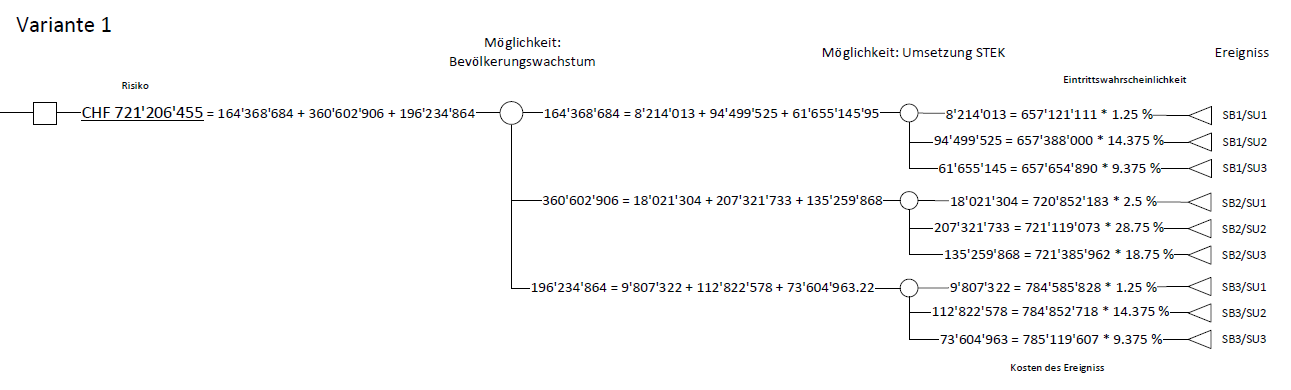
\includegraphics[width=\textwidth]{figures/f-04-08-01-Risikoberechnung}
	\caption[Risikoberechnung]{Beispiel der Risikoberechnung}
	\label{img:Risikoberechnung}
\end{figure}




% ===========================================================================
% EOF
%

%%% Local Variables:
%%% mode: latex
%%% TeX-master: "../main"
%%% End:




	\subsection{Sensitivitätsanalyse}
	\input{content/Fallstudie/04-09-Sensitivitätsanalyse}

% ===========================================================================
% EOF
%

%%% Local Variables:
%%% mode: latex
%%% TeX-master: "../main"
%%% End:
